\documentclass[11pt, oneside]{article} 
\usepackage{amsmath, amsthm, amssymb, calrsfs, wasysym, verbatim, bbm, color, graphics, graphicx, geometry}
\usepackage[most]{tcolorbox}
\usepackage{xcolor}
\usepackage{framed}
\usepackage{caption}
\usepackage{subcaption}
%\colorlet{shadecolor}{blue!15}
\graphicspath{ {./figs} }

\geometry{tmargin=.75in, bmargin=.75in, lmargin=.75in, rmargin = .75in}  

\newcommand{\R}{\mathbb{R}}
\newcommand{\C}{\mathbb{C}}
\newcommand{\Z}{\mathbb{Z}}
\newcommand{\N}{\mathbb{N}}
\newcommand{\Q}{\mathbb{Q}}
\newcommand{\Cdot}{\boldsymbol{\cdot}}

%\newtheorem{thm}{Theorem}
%\newtheorem{defn}{Definition}
%\newtheorem{conv}{Convention}
%\newtheorem{rem}{Remark}
%\newtheorem{lem}{Lemma}
%\newtheorem{cor}{Corollary}
%\newtheorem{exa}{Ejemplo}

\newtcbtheorem[auto counter]{eje}%
  {Ejemplo}{fonttitle=\bfseries\upshape, fontupper=\slshape,
     arc=0mm, colback=blue!5!white,colframe=blue!75!black}{Ejemplo}

\newtcbtheorem[auto counter]{alg}%
  {Algoritmo}{fonttitle=\bfseries\upshape, fontupper=\slshape,
     arc=0mm, colback=red!5!white,colframe=red!75!black}{Algoritmo}

\title{Estructuras Hidr\'aulicas [2015961] \\ \textbf{Tema \# 1: Conceptos b\'asicos}}
\author{\textbf{Luis Alejandro Morales (Ph.D)}\\ \vspace{0.4cm} Profesor Asistente \\ Universidad Nacional de Colombia-Bogot\'a\\Facultad de Ingenier\'ia \\ Departamento de Ingenieria Civil y Agr\'icola}
%\date{Periodo 2022-II}
\date{}

\begin{document}

\maketitle
\tableofcontents

%\vspace{.25in}

%%%%%%%%
\section{Introducci\'on} % From VChow
\subsection{Generalidades}
En general el flujo de fluidos se presenta como \emph{flujo a presi\'on} (flujo en tuber\'ias) y el \emph{flujo a superficie libre} (flujo en canales). La diferencia entre estos tipos de flujo es que en un canal la superficie del flujo est\'a en contacto con el aire y por lo tanto somet\'ido a una presi\'on atmosf\'erica. En el caso del flujo a presi\'on, la secci\'on de la tuber\'ia est\'a totalmente copada por el fluido y por lo tanto sobre el flujo se ejerce, adem\'as de una presi\'on atmosf\'erica sobre el conducto, una presi\'on hidr\'aulica. Analisando la figura~\ref{fig1}, se que la \emph{linea de gradiente hidr\'aulica {LGH}} para el flujo en tuber\'ias est\'a conformada por el nivel topogr\'afico del eje central de la tuber\'ia ($z$) y la presi\'on del flujo medida con los piez\'ometros ($\frac{p}{\gamma}$), mientras que en el flujo a superficie libre el termino de la presi\'on es equivalente a la profundidad del flujo ($y$). En la tuber\'ia la linea de gradiente hidr\'aulica est\'a formada por $z + \frac{p}{\gamma}$, en el canal esta formada por $z+y$. 
% VChow fig 1.1
\begin{figure}[h]
\centering
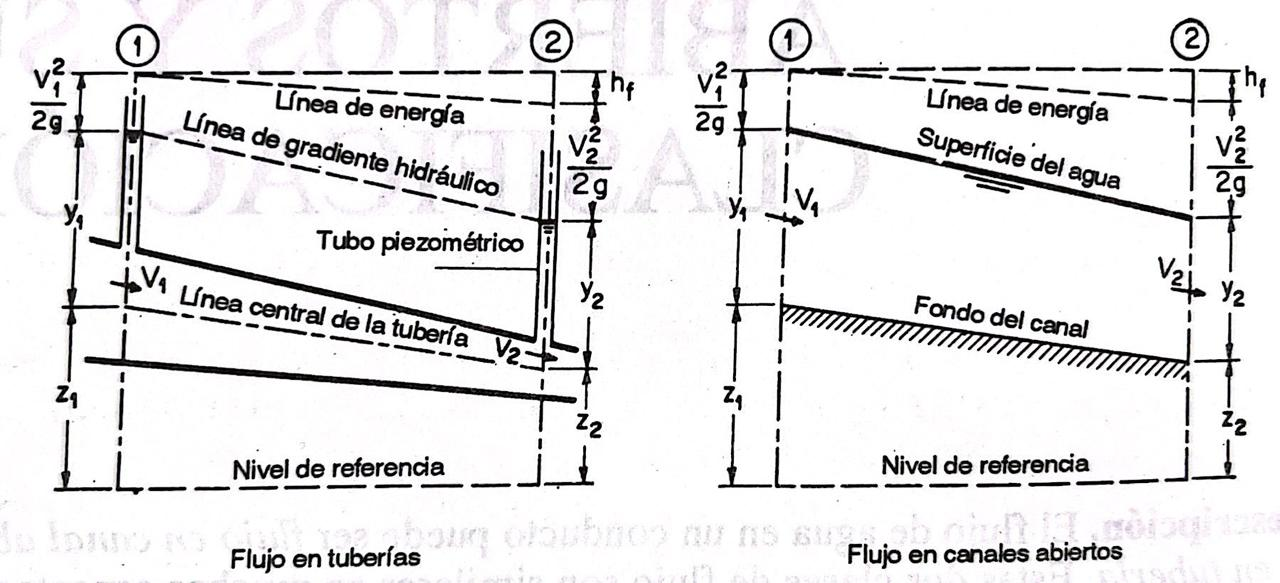
\includegraphics[width=0.9\textwidth]{fig1.jpeg}
\caption{Linea de gradiente hidr\'aulico y de energ\'ia en a) flujo a presi\'on y b) flujo a superficie libre (tomado de \cite{VChow}).}
\label{fig1}
\end{figure}

Cabe aclarar que el an\'alisis del flujo en canales es m\'as complejo que el flujo. Mientras que en una tuber\'ia la secci\'on que atraviesa el flujo es constante y determinada por la geometr\'ia de la tuber\'ia que es muchas veces circular, en un canal la secci\'on puede tomar muchas formas geom\'etricas e inclusive puede ser totalmente irregular como en el caso de canales naturales. Por otro lado, la presi\'on en una tuber\'ia de secci\'on constante no cambia en el tiempo mientras que en un canal la profundidad  del flujo cambia cuando cambia la pendiente del canal. Esto hace que las pendientes de la superficie del agua y del fondo del canal sean diferentes. Adem\'as, mientras que la rugosidad en una tuber\'ia es independiente de las condiciones de flujo, la rugosidad en un canal depende del nivel de agua. Todos estos factores hacen que el flujo en canales sea m\'as incierto y recurra m\'as al uso de ecuaciones emp\'iricas y al conocimiento previo de otras disciplinas como la \emph{hidrolog\'ia} y la \emph{geomorfolog\'ia}.

\subsection{Tipos de canales}
Un canal es un conducto en el cual el agua fluye con su superficie libre (en contacto con la atmósfera). Los canales pueden ser clasificados como:
\begin{itemize}
\item \textbf{Naturales}: Son aquellos cursos naturales de agua que existen sobre la tierra. Se pueden clasificar como arroyos o quebradas que existen en zonas montañosas hasta r\'ios y estu\'arios, los cuales poseen dimensiones mucho mayores y existen en llanuras y en desembocaduras a océanos y mares, respectivamente. Debido a su irregularidad, las propiedades hidr\'aulicas de los canales naturales cambian continuamente en el espacio y en el tiempo. 
\item \textbf{Artificiales}: Son aquellos construidos por el ser humano cuyas formas suelen ser de geometr\'ia conocida. Estos canales  se construyen para la navegaci\'on, en centrales hidroel\'ectricas, en sistemas de riego, en drenajes en v\'ias, para vertederos y tomas de agua, y en laboratorios para el estudio del flujo. Se han encontrado que las teor\'ias hidr\'aulicas desarrolladas para canales artificiales se pueden aplicar a canales naturales con un buen grado de aproximaci\'on.  Existen tipos de canales artificiales:

\begin{itemize}
\item \emph{Canal}: Canal excavado en el sitio generalmente revestido con pasto, concreto, ladrillo o asfalto. Usualmente tienen bajas pendientes y son utilizados en el drenaje urbano.
\item \emph{Canaleta}: Canal de menor tamaño que el canal y apoyado sobre el terreno. Suelen construirse en metal, mamposter\'ia o concreto y sirven para transportar el agua  a trav\'es de una depresi\'on. 
\item \emph{Rápidas y Caídas}: Son canales de alta pendiente construidos en longitudes cortas. 
\item \emph{Alcantarilla}: Es un canal cerrado, generalmente de secci\'on circular y longitud corta, construido en concreto o mampostería que sirve para el drenaje de aguas servidas y lluvias en sistemas urbanos. 
\item \emph{T\'uneles}: Canales no revestidos y excavados en roca, y revestidos en concreto o mamposter\'ia comúnmente usados en centrales hidroel\'ectricas. 
\end{itemize}
\end{itemize}


\begin{figure}
     \centering
     \begin{subfigure}[b]{0.48\textwidth}
         \centering
         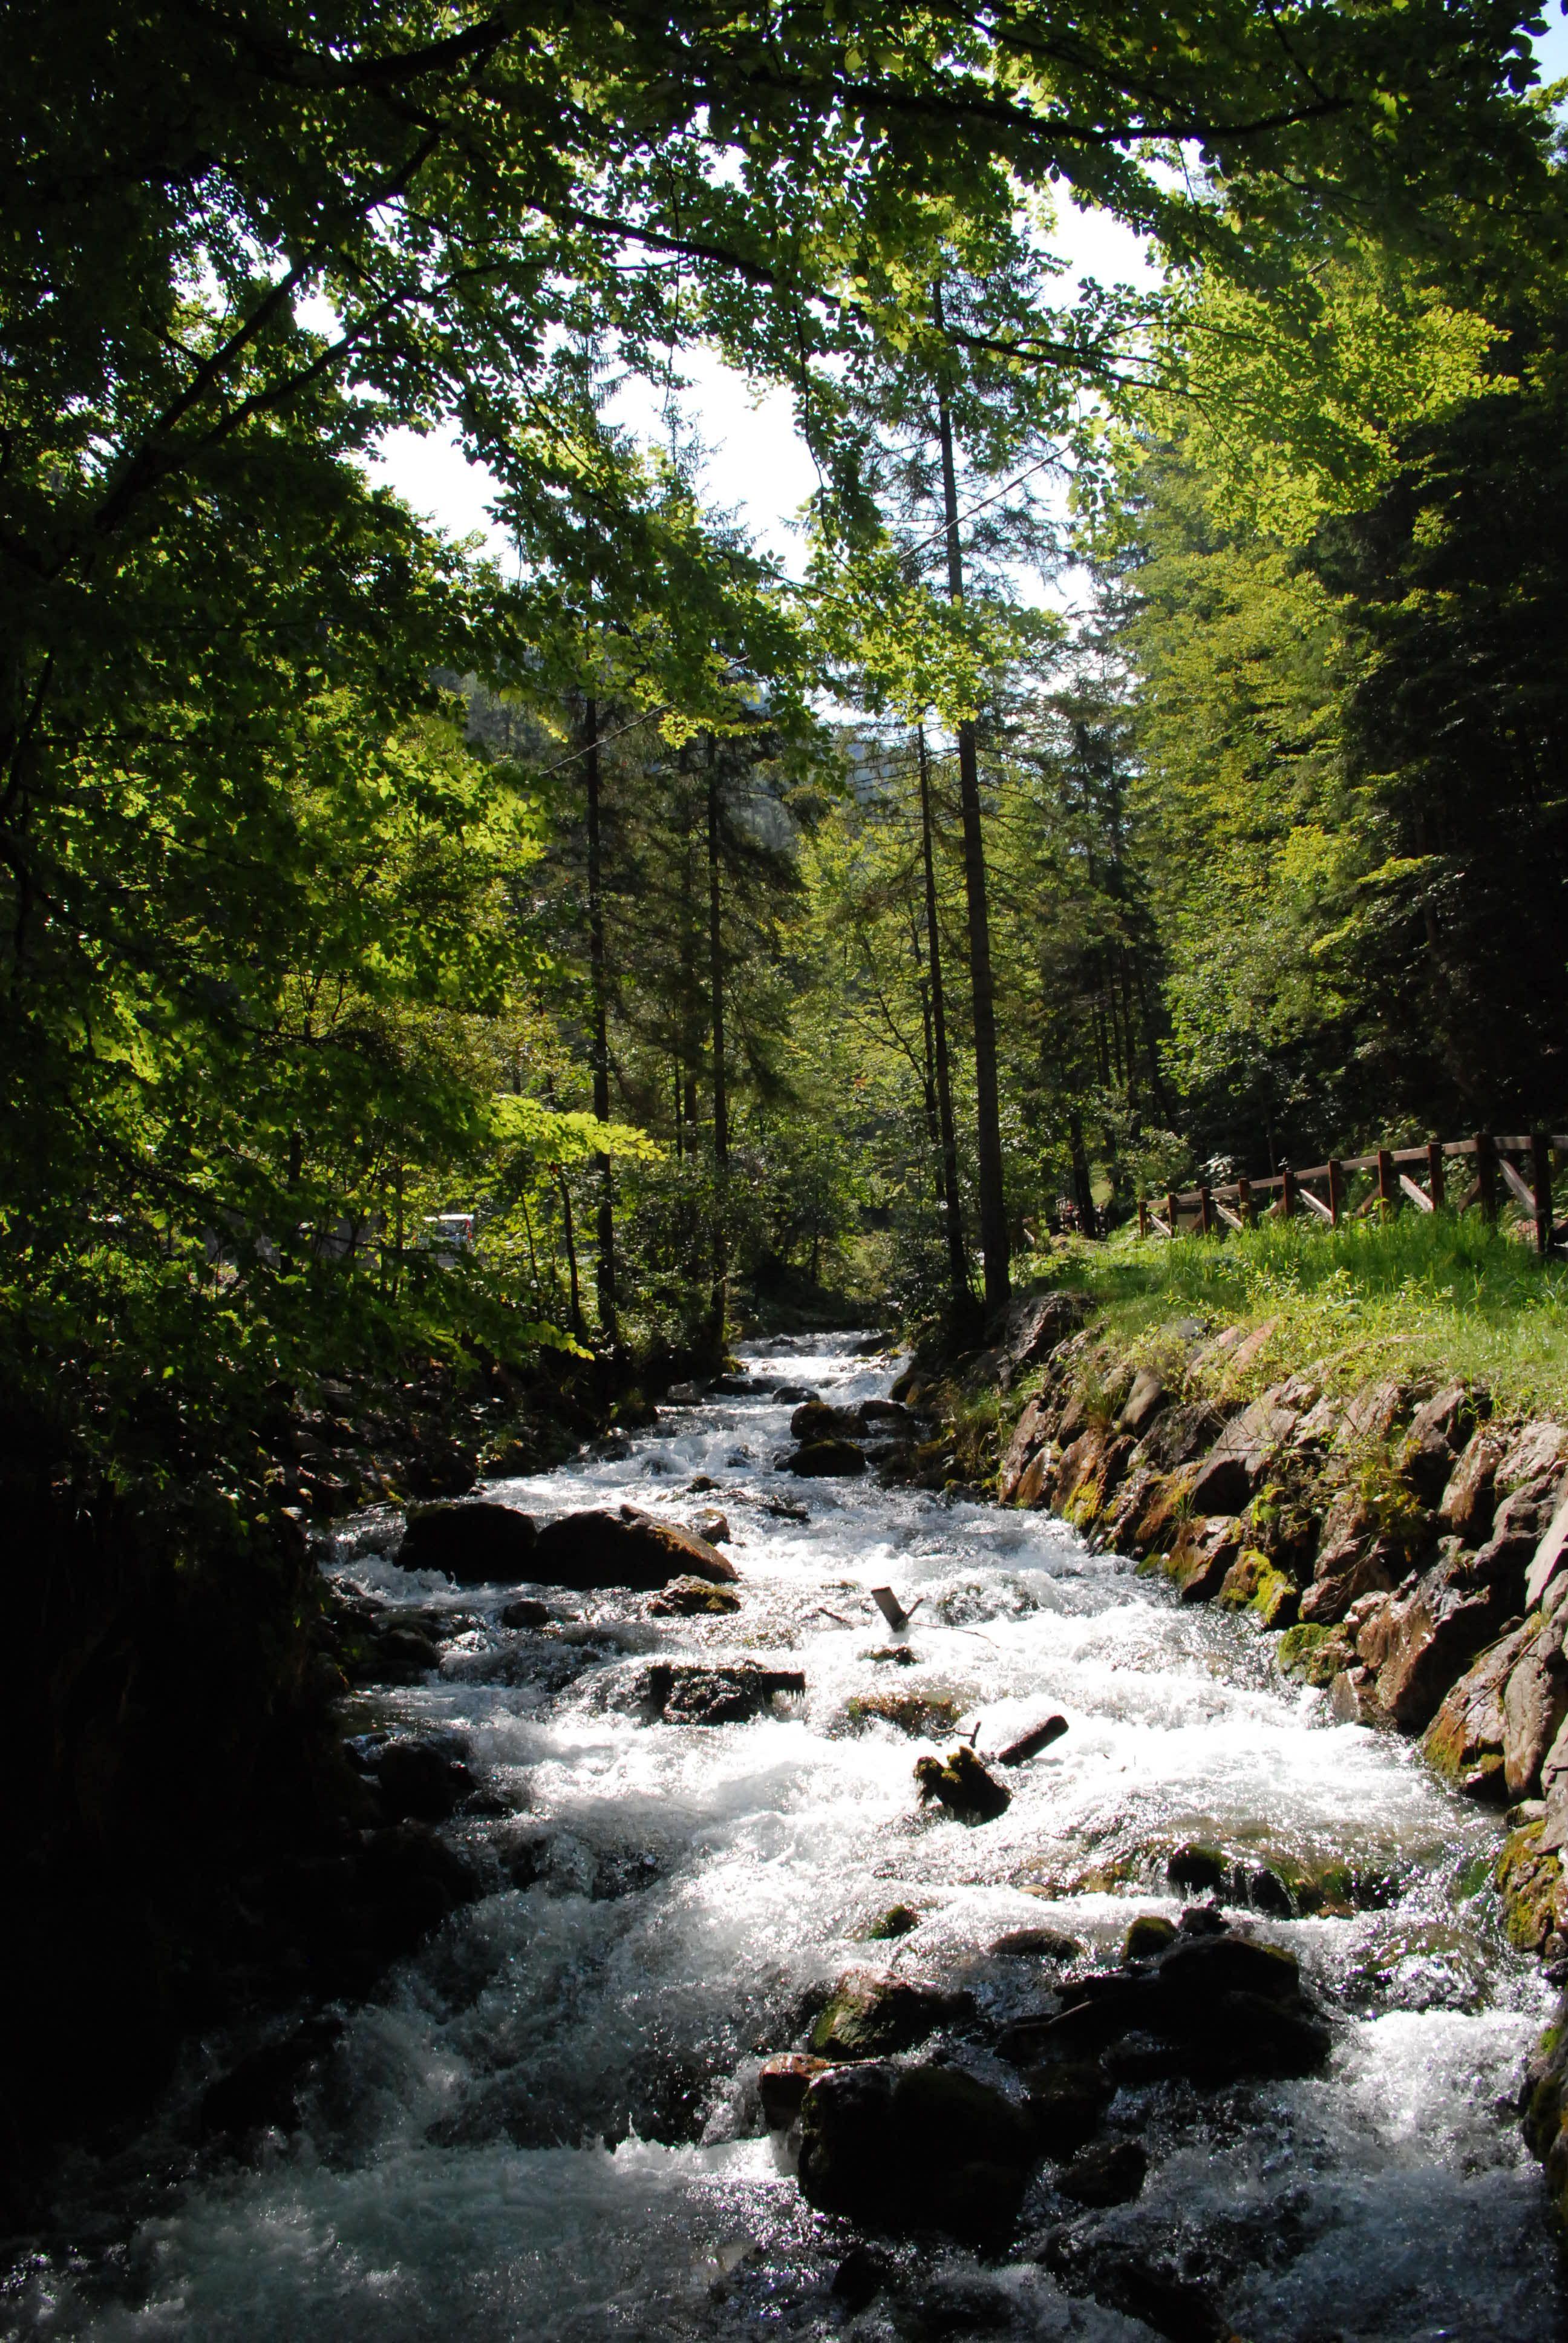
\includegraphics[width=\textwidth]{fig2a}
         \caption{Quebrada de alta montaña}
         \label{fig2a}
     \end{subfigure}
     \hfill
     \begin{subfigure}[b]{0.48\textwidth}
         \centering
         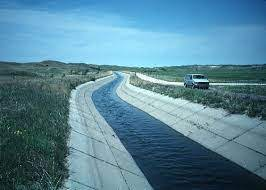
\includegraphics[width=\textwidth]{fig2b}
         \caption{Canal artificial}
         \label{fig2b}
     \end{subfigure}
      \caption{Tipos de canales principales.}
      %\label{fig:three graphs}
\end{figure}

\begin{figure}
     \centering
     \begin{subfigure}[b]{0.32\textwidth}
         \centering
         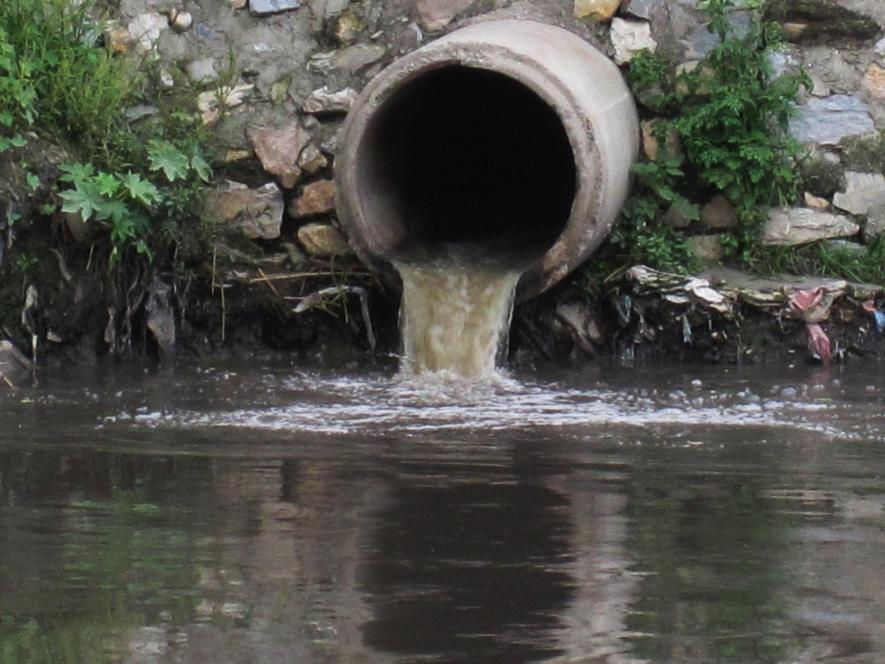
\includegraphics[width=\textwidth]{fig21a}
         \caption{Alcantarilla}
         \label{fig21a}
     \end{subfigure}
     \hfill
     \begin{subfigure}[b]{0.32\textwidth}
         \centering
         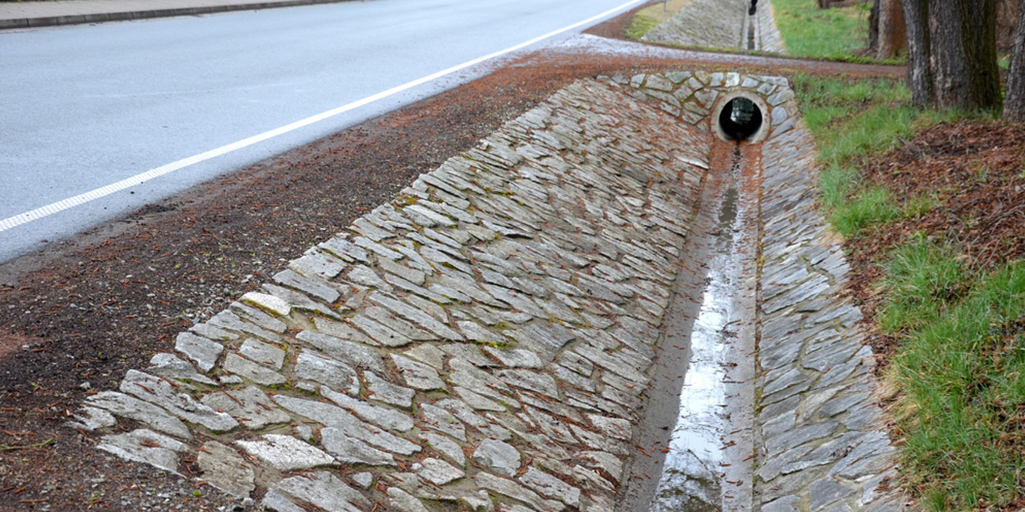
\includegraphics[width=\textwidth]{fig21b}
         \caption{Cuneta en una v\'ia}
         \label{fig21b}
     \end{subfigure}
     \hfill
     \begin{subfigure}[b]{0.32\textwidth}
         \centering
         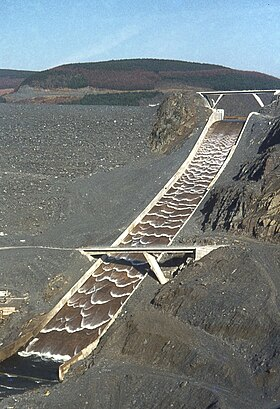
\includegraphics[width=\textwidth]{fig21c.jpg}
         \caption{Vertedero en una presa}
         \label{fig21c}
     \end{subfigure}
       \caption{Tipos de canales artificiales.}
      %\label{fig:three graphs}
   \end{figure}

\subsection{Geometr\'ia de un canal}
Un \emph{canal prismático} es aquel cuya sección transversal y pendiente permanecen constantes mientras que un \emph{canal no prismático} es aquel en donde la sección y/o la pendiente cambian a lo largo de su longitud (e.g. vertedero de ancho variable). La sección de un canal, es la sección en la dimensión transversal o perpendicular a la direcci\'on de flujo. En  canales naturales la secci\'on transversal es irregular y cambia en el espacio y en el tiempo. Cuando ocurren crecientes, generalmente el canal central transporta la mayoría del flujo mientras los canales en las bancas transportan menor flujo.

Los canales artificiales tienen geometr\'ias como las que se muestran en la figura~\ref{fig3}. Los canales abiertos m\'as comunes son los rectangulares y los trapezoidales. Los canales circulares son los mas comunes en sistemas de alcantarillado. Existen otras formas de canales cerrados como la secci\'on rectangular, en forma de ovalo o de herradura. En muchos estudios de cauces naturales la par\'abola se utiliza como una aproximaci\'on a una secci\'on de un canal natural. 

% VChow fig 2.1
\begin{figure}[h]
\centering
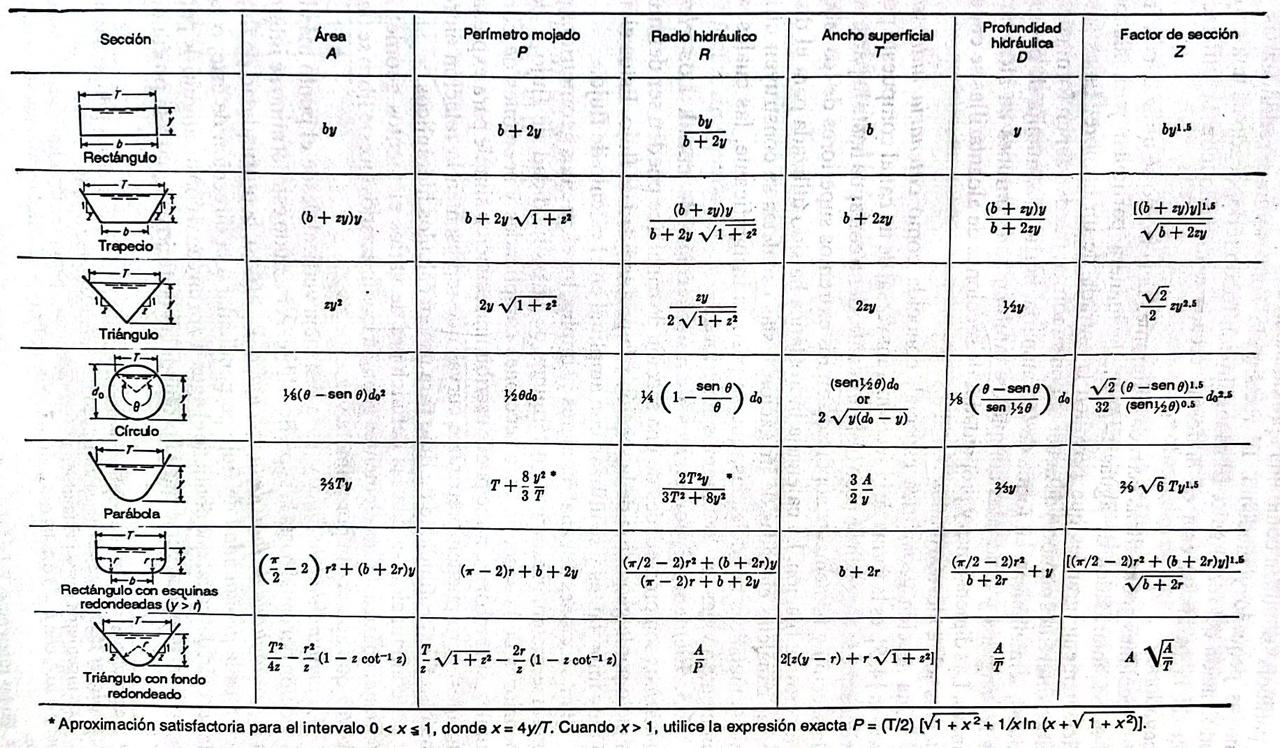
\includegraphics[width=\textwidth]{fig3.jpeg}
\caption{Geometr\'ias y elementos geom\'etricos de secciones transversales de un canal (tomado de \cite{VChow}).}
\label{fig3}
\end{figure}

Las \emph{propiedades geom\'etricas} (ver figura~\ref{fig3}) de un canal se expresan a través de ecuaciones en funci\'on de la profundidad del flujo y de otras dimensiones de la secci\'on. Sin embargo para el caso de canales naturales, no es posible obtener ecuaciones y es necesario el uso de m\'etodos num\'ericos para obtener dichas propiedades. Las propiedades geom\'etricas m\'as importantes son las siguientes:
\begin{itemize}
\item \textbf{profundidad de flujo ($y$)}: es la distancia vertical desde el punto mas bajo de la secci\'on hasta la superficie del agua. 
\item \textbf{profundidad de la secci\'on ($d$)}: es la distancia perpendicular al flujo desde el punto mas bajo de la sección hasta la superficie del agua. $y=\frac{d}{\cos \theta}$ donde $\theta$ es el angulo de la pendiente longitudinal del canal. 
\item \textbf{nivel ($z$)}: es la elevaci\'on de la superficie del agua desde un nivel de referencia o datum. Si el nivel de referencia es el fondo, $z=y$.
\item  \textbf{ancho superficial ($T$)}: ancho de la secci\'on transversal en la superficie libre. 
\item  \textbf{\'area mojada ($A$)}: es el \'area de la secci\'on transversal en contacto con el fluido perpendicular a la direcci\'on del flujo. 
\item  \textbf{perímetro mojada ($P$)}: es el per\'imetro de la secci\'on transversal en contacto con el fluido.
\item  \textbf{radio hidr\'aulico ($R$)}: es la relaci\'on entre el per\'imetro mojado y el \'area mojada, $R=\frac{A}{P}$.
\item  \textbf{profundidad hidr\'aulica ($D$)}: es  $D=\frac{A}{T}$.
\item  \textbf{factor de secci\'on ($Z$)}: para el c\'alculo del \emph{flujo cr\'itico}, se calcula como $Z= A\sqrt{D} = A \sqrt{\frac{A}{T}}$. Para el caso de \emph{flujo uniforme} $Z=AR^{(2/3)}$.
\end{itemize}

%%%%%%%%
\section{Clasificaci\'on y reg\'imenes de flujo} % From Chau 
Con base en diferentes criterios, el flujo a superficie libre se puede clasificar en diferentes tipos (ver figura~\ref{fig4}).

% Chau fig 1.7
\begin{figure}[h]
\centering
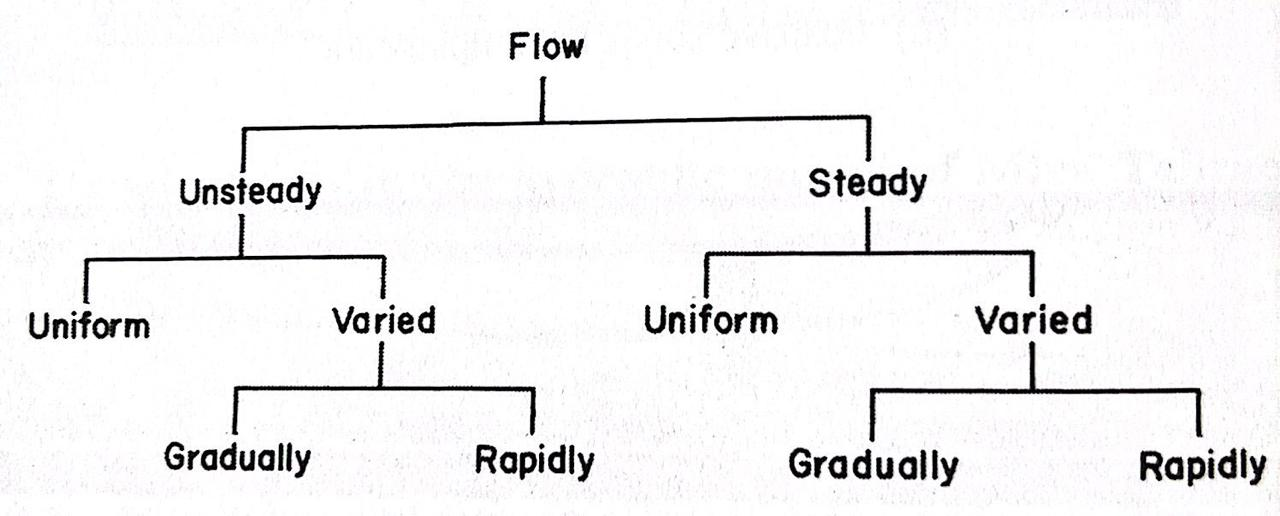
\includegraphics[width=\textwidth]{fig4.jpeg}
\caption{Clasificaci\'on de flujos a superficie libre (tomado de \cite{Chau}).}
\label{fig4}
\end{figure}

\subsection{Flujo permanente y no permanente}
Si la velocidad del flujo ($\vec{U}= u\vec{i} + v\vec{j} + w\vec{k}$) en un punto determinado del espacio dentro del flujo no cambia en el tiempo $t$, el flujo es \emph{permanente}. Si la velocidad del flujo cambia en un punto determinado del espacio con respecto al el tiempo, el flujo es no \emph{permanente}. Esto quiere decir que el termino de la \emph{aceleración local} ($\partial{\vec{U}}/\partial{t}$), en el campo vectorial de la aceleración ($\vec{a}$), es igual a cero (el cambio de las tres componentes de $\vec{U}$ con respecto al tiempo es cero). Es posible transformar el flujo no permanente en flujo permanente si el sistema de referencia se mueve con el flujo, e.g. con una onda de creciente que no cambia de forma.  

\subsection{Flujo uniforme y no uniforme}
Si la velocidad del flujo para un instante de tiempo $t$ no cambio a lo largo de un tramo de canal ($\vec{l} = x\vec{i} + y\vec{j} + z\vec{k}$), el \emph{flujo es uniforme}. Esto quiere decir que el \emph{termino convectivo} ($\vec{U} ( \vec{\nabla} \cdot \vec{U} )$) del  campo vectorial de la aceleraci\'on es igual a cero. Note que el operador $\vec{\nabla}=\frac{\partial}{\partial x} \vec{i} + \frac{\partial}{\partial y} \vec{j} + \frac{\partial}{\partial z} \vec{k}$. Esta condici\'on de flujo uniforme se cumple para la velocidad media de una secci\'on. Sin embargo se considera flujo uniforme incluso cuando la velocidad en diferentes puntos de una secci\'on no es la misma. 

Cuando la velocidad para un instante de tiempo dado cambia a lo largo de un tramo de canal, el flujo se considera \emph{no uniforme} o \emph{variado}. Dependiendo de la variación a lo largo del canal, el flujo se puede clasificar como \emph{gradualmente variado} o \emph{rápidamente variado}. En un flujo gradualmente variado, la profundidad de flujo varia gradualmente a lo largo de la distancia mientras que en un flujo rápidamente variado la profundidad varia rápidamente para una distancia corta.

De acuerdo con lo anterior, para flujo permanente y uniforme, la velocidad no varia ni con con el espacio ni con el tiempo, esto quiere decir que el campo vectorial de la aceleración (derivada total de la velocidad con respecto al tiempo) es igual a cero $\vec{a}=\frac{d \vec{U}}{d t} = 0$.

\subsection{Flujo laminar y flujo turbulento}
El flujo es \emph{laminar} cuando las partículas de fluido se desplazan de manera organizada formando capas que se mueven unas sobre otras. En un flujo \emph{turbulento} las partículas de fluido se mueven de manera ca\'otica en trayectorias irregulares. Analizando las fuerzas que intervienen en el flujo de fluidos, el flujo es laminar cuando las fuerzas dominantes son las \emph{fuerzas viscosas} y es turbulento cuando las fuerzas dominantes son las \emph{fuerzas inerciales}. La clasificaci\'on de un flujo en laminar o turbulento, se hace a trav\'es del \emph{numero de Reynolds} ($R_e$):
\begin{equation}
R_e = \frac{\text{fuerzas inerciales}}{\text{fuerzas viscosas}} = \frac{V L}{\nu}
\label{Re}
\end{equation}
donde $V$ es la velocidad media de la secci\'on, $\nu$ es la viscosidad cinem\'atica del fluido y $L$ es una longitud característica que para flujo a superficie libre es igual al radio hidráulico $R$ o la profundidad hidráulica. Para flujo en canales, la transición de flujo laminar a turbulento ocurre cuando $R_e \approx $ 600. Flujo laminar a superficie libre es muy raro en la vida real. Sin embargo en modelos a escala, es posible que para profundidades de flujo pequeñas  se presente flujo laminar en el modelo cuando en realidad el flujo en el prototipo es turbulento. 

\subsection{Flujo subcr\'tico, cr\'itico y supercr\'itico}
Un flujo es \emph{cr\'itico} cuando este tiene una velocidad media igual a la velocidad con la que se desplaza una onda de gravedad de pequeña amplitud en el flujo. La onda de gravedad se forma por cambios en la profundidad del flujo. Un flujo es \emph{subcr\'itico} cuando la velocidad media es menor que la \emph{velocidad cr\'tica} y es \emph{supercr\'itico} cuando la velocidad media es mayor que la velocidad cr\'itica. Para la clasificaci\'on de estos tipos de flujo, se utiliza el \emph{n\'umero de Froude} ($R_r$):
\begin{equation}
F_r = \frac{\text{fuerzas inerciales}}{\text{fuerzas gravitacionales}} = \frac{V}{\sqrt{g L}}
\label{Fr}
\end{equation}
donde $g$ es la aceleraci\'on de la gravedad y $L$ es una longitud característica igual a la profundidad hidráulica $D$ que para canales rectangulares es $D=y$. De acuerdo con la ecuacio~\ref{Fr}, el flujo es cr\'tico cuando $F_r = 1$, es subcr\'itico cuando $F_r < 1$ y es supercr\'itico cuando $F_r > 1$.

Pueden presentarse combinaciones de tipos de flujo de acuerdo con el valor de $R_e$ y de $F_r$ como: \emph{subcr\'itico laminar}, \emph{subcr\'itico turbulento}, \emph{supercr\'itico laminar} y \emph{supercr\'itico turbulento} (ver figura~\ref{fig41})

% VChow fig 1.5
\begin{figure}[h]
\centering
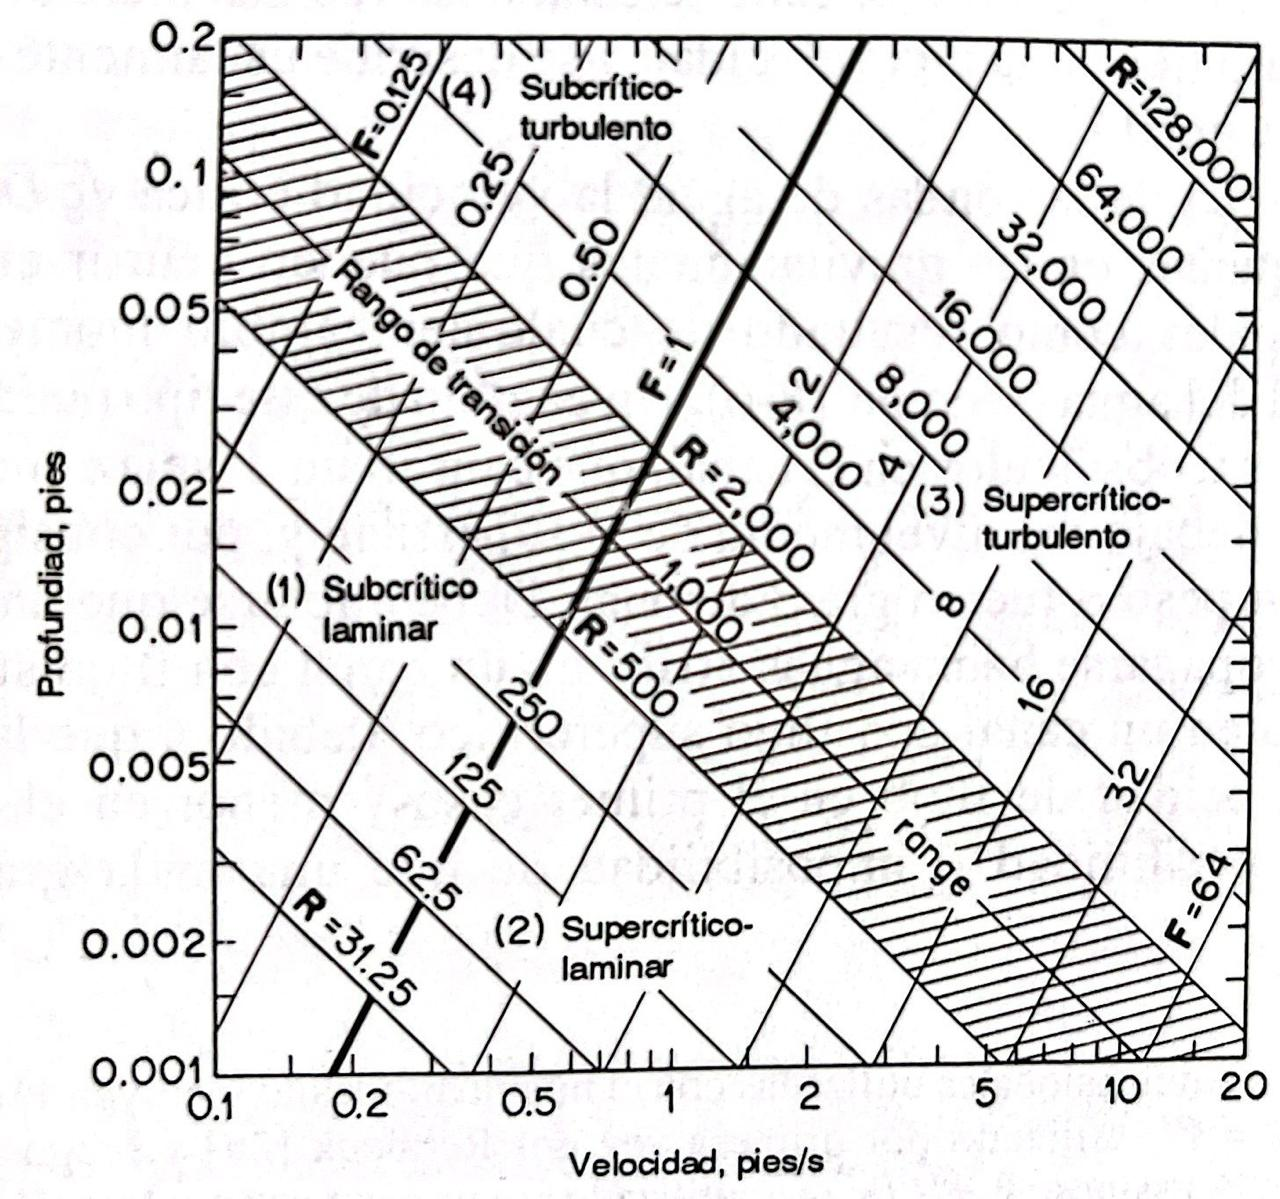
\includegraphics[width=0.9\textwidth]{fig41.jpeg}
\caption{Profundidad vs velocidad para cuatro regímenes flujo en canales abiertos anchos. Note que las escalas son logarítmicas (tomado de \cite{VChow}).}
\label{fig41}
\end{figure}

Los flujos subcr\'itico laminar y supercr\'itico laminar son poco comunes en la naturales y se presentan cuando la profundidad de agua es pequeña lo cual suele ocurrir en modelos a escala. En casos reales los flujos son turbulentos.

%%%%%%%%
\section{Distribuci\'on de velocidades}% From Chau 
La velocidad del flujo en una secci\'on de canal varia en cada punto dentro de esta debido a los esfuerzos cortantes entre capas de flujo inducidas por la rugosidad ejercida por el fondo y las bancas del canal, y por la superficie libre en contacto con el aire (ver figura~\ref{fig5}).

% Chau fig 1.9
\begin{figure}[h]
\centering
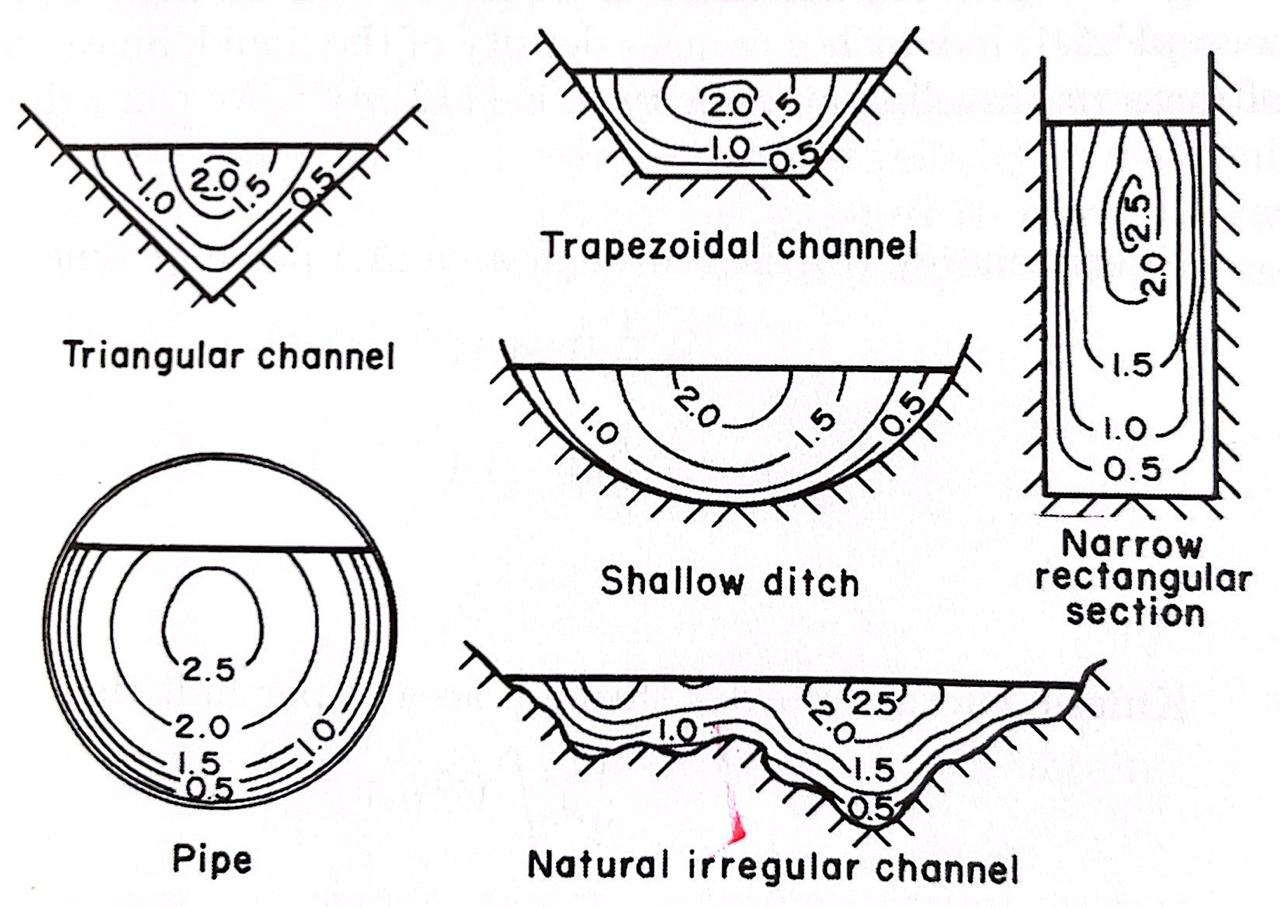
\includegraphics[width=0.9\textwidth]{fig5.jpeg}
\caption{Distribuci\'on de velocidad de flujo en diferentes tipos de canales (tomado de \cite{Chau}).}
\label{fig5}
\end{figure}


En teor\'ia la velocidad varia en las tres dimensiones espaciales. Sin embargo en la practica, los mayores gradientes de velocidad se dan a lo largo de la direcci\'on del flujo. 
% VChow fig 2.5
\begin{figure}[h]
\centering
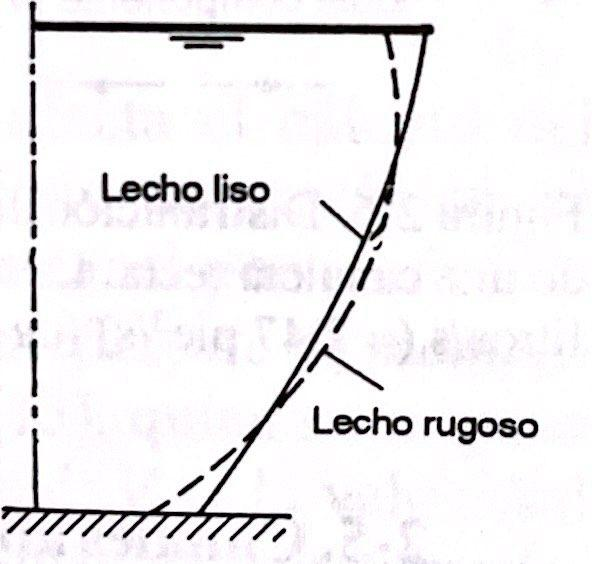
\includegraphics[width=8cm]{fig6.jpeg}
\caption{Distribuci\'on de velocidades en un canal liso y rugoso (tomado de \cite{VChow}).}
\label{fig6}
\end{figure}

\subsection{Coeficiente de energ\'ia}
%Teniendo en cuenta que la velocidad cambia en cualquier punto en una seccion transversal de un canal, la cabeza de velocidad promedio ($\left( \frac{U^2}{2g} \right)_m$) es diferente a la ccabeza de velocidad estimada con la velocidad media ($\frac{V^2}{2g}$). 
Si analizamos un flujo de fluido de densidad $\rho$ cuyo campo de velocidades es $\vec{U}$ que pasa a través de una sección infinitesimal $dA$, la energ\'ia cinem\'atica del flujo por unidad de tiempo es $\frac{1}{2}\rho dA U^3$. La energ\'ia cinem\'atica del flujo a partir de la velocidad media en la sección $V$, se puede estimar como  $\frac{1}{2}\rho dA V^3$. Sin embargo estas dos maneras de calcular la energ\'ia cinem\'atica por unidad de tiempo no son equivalentes. Para superar estas diferencias, se introduce un \emph{coeficiente de energía} o \emph{coeficiente de Coriolis} en la segunda ecuaci\'on, quedando $\frac{1}{2}\alpha \rho dA V^3$. Igualando las dos ecuaciones e integrando para el área $A$ de la sección transversal, se tiene:

$$
\frac{1}{2}\alpha\rho V^3 \int_A dA  = \frac{1}{2}\rho \int_A U^3 dA 
$$
Simplificando y despejando para $\alpha$, se tiene que:

\begin{equation}
\alpha = \frac{\int_A U^3 dA}{V^3 \int_A dA}
\label{alp}
\end{equation}

Teniendo en cuenta que la velocidad media en la secci\'on de flujo $V$ se calcula como $V=\frac{1}{A}\int_A U dA$, reemplazando en la ecuaci\'on~\ref{alp}, tenemos:

\begin{equation}
\alpha = \frac{A^3 \int_A U^3 dA}{\left(\int_A U dA \right)^3 \int_A dA}= \frac{A^2 \int_A U^3 dA}{\left(\int_A U dA \right)^3 }
\label{alp2}
\end{equation}

La forma discreta de la ecuaci\'on anterior, se expresa como:

\begin{equation}
\color{red}\boxed{\color{black} \alpha = \frac{\sum_{i=1}^{N}A_i^2 \sum_{i=1}^{N} U_i^3 A_i} {\left(\sum_{i=1}^{N} U_i A_i \right)^3 }}
\label{alp3}
\end{equation}

donde $N$ es el numero de subsecciones verticales en las cuales una secci\'on es dividida, $A_i$ es el área de la subsecci\'on $i$ y $U_i$ es la velocidad media en la subsecci\'on $i$.

\subsection{Coeficiente de cantidad de movimiento}
El flujo de cantidad de movimiento por unidad de tiempo a trav\'es de una secci\'on $dA$ cuyo campo de velocidad es $\vec{U}$ es $\frac{1}{2}\rho dA U^2$. Si tomamos la velocidad media en la secci\'on $V$, el flujo de cantidad de movimiento a trav\'es de $dA$ por unidad de tiempo es $\frac{1}{2}\rho dA V^2$. Para que estas dos ecuaciones sean equivalentes, la \'ultima ecuaci\'on se debe multiplicar por un \emph{coeficiente de cantidad de movimiento} ($\beta$), quedando $\frac{1}{2}\beta \rho dA V^2$. Igualando estas dos ecuaciones e integrando para $A$, se tiene:

$$
\frac{1}{2}\beta\rho V^2 \int_A dA  = \frac{1}{2}\rho \int_A U^2 dA 
$$

Simplificando y despejando para $\alpha$, se tiene que:
\begin{equation}
\beta = \frac{\int_A U^2 dA}{V^2 \int_A dA}
\label{bet}
\end{equation}

Reemplazando para $V$ en la ecuaci\'on~\ref{bet}, se tiene:
\begin{equation}
\beta = \frac{A \int_A U^2 dA}{\left(\int_A U dA \right)^2 }
\label{bet2}
\end{equation}

La forma discreta de la ecuaci\'on anterior, se expresa como:

\begin{equation}
\color{red}\boxed{\color{black} \beta = \frac{\sum_{i=1}^{N}A_i \sum_{i=1}^{N} U_i^2 A_i} {\left(\sum_{i=1}^{N} U_i A_i \right)^2 }}
\label{bet3}
\end{equation}

Valores teóricos de $\alpha$ y $\beta$ se pueden deducir a partir de la \emph{ley de potencia} o de la \emph{ley logarítmica} de distribuci\'on de velocidades en canales anchos. Algunos valores típicos de $\alpha$ y $\beta$ para diferentes secciones de canal, se relacionan la tabla~\ref{tab1}. En términos generales para canales prismáticos y circulares rectos, los valores de $\alpha$ y $\beta$ son menores a 1.15 y aproximadamente igual a 1.0.

% Chau tab 1.2
\begin{table}[h!]
\centering
\begin{tabular}{l c c}
 \hline
 Secci\'on de canal & $\alpha$ & $\beta$ \\ [0.5ex]
 \hline\hline
Canales regulares & 1.10-1.20 & 1.03-1.07 \\
Canales naturales & 1.15-1.50 & 1.05-1.17 \\
R\'ios cubiertos de hielo & 1.20-2.00 & 1.07-1.33 \\
Llanuras de inundaci\'on & 1.50-2.00 & 1.17-1.33 \\
\hline
\end{tabular}
\caption{Coeficientes $\alpha$ y $\beta$ para diferentes tipos de secci\'on (tomado de \cite{Chau}).}
\label{tab1}
\end{table}

%%%%%%%%
\section{Distribuci\'on de presiones}% From Chau 
La distribuci\'on de presiones en un canal depende de las condiciones de flujo. A continuaci\'on se analisar\'a las distribuciones para diferentes condiciones.

\subsection{Fluido est\'atico}
En el caso de un fluido est\'atico, si se analizan las fuerzas ejercidas sobre una porci\'on del fluido de \'area transversal $dA$ y altura $y$, se tiene que las fuerzas en el plano horizontal se cancelan, por lo que las únicas fuerzas actuantes son el eje vertical $z$. Haciendo sumatoria de fuerzas en $z$ igual a cero (fluido estático sin aceleraci\'on) y trabajando en términos de presiones manométricas, tenemos que:
$$
f_z = w
$$
donde $w$ es el peso del elemento de fluido fluido $W=\rho g y dA$ y $f_z$ es la fuerza de presi\'on hidro estática $p$ ejercida  por el fluido sobre $dA$ por lo que $f_z = p dA$. Reemplazando y simplificando, tenemos:

$$
p=\rho g y
$$
Esta ecuaci\'on determina la presi\'on manométrica en un fluido incompresible ($\rho$ es constante) en reposo a una profundidad $y$. Note que a grandes profundidades $\rho$ cambia por lo que la ecuaci\'on anterior no se cumple.

\subsection{Flujo horizontal y paralelo}
Consideremos ahora un fluido que se mueve en capas en un canal horizontal sin fricci\'on. Si  no existe aceleración del fluido en la direcci\'on del flujo y si la velocidad es uniforme en la secci\'on y paralela al fondo del canal, la sumatoria de fuerzas en la direcci\'on del flujo es cero. Las fuerzas actuantes son a lo largo del eje vertical las cuales son la fuerza de presi\'on hidroest\'atica a una profundidad $y$ y el peso del elemento de fluido $w$. Similar al caso de fluido est\'atico, tenemos entonces que:

$$
p=\rho g y
$$
 
\subsection{Flujo paralelo en un canal inclinado}
Consideremos el flujo en un canal con una pendiente dada por el angulo $\theta$ (ver figura~\ref{fig7}). Si no existe aceleraci\'on del fluido en direcci\'on del flujo y si la velocidad es uniforme en la secci\'on del canal y paralela al fondo de este, las fuerzas actuantes son a lo largo del eje del elemento y su sumatoria es igual a cero. El peso  $w=\rho g d dA$ en direcci\'on vertical hacia abajo, al proyectarlo sobre el eje del elemento se tiene $w=\rho g dA \cos \theta d$; note que $d$ es la profundidad de la secci\'on. La otra fuerza a lo largo del eje del elemento es la fuerza de presi\'on $f_z=p dA$. Teniendo en cuenta que $d= y \cos \theta$, el peso del elemento de fluido se convierte en $w = \rho g y \cos^2 \theta$. Haciendo sumatoria de fuerzas a lo largo del eje del elemento, se tiene:

$$
p=\rho g y \cos^2 \theta
$$

% Chau fig 1.15
\begin{figure}[h]
\centering
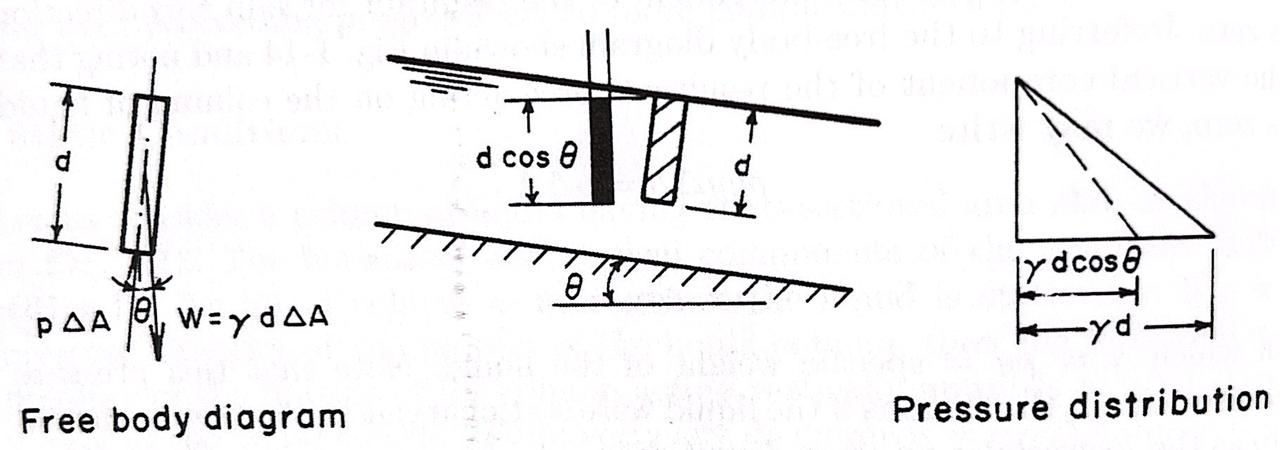
\includegraphics[width=0.9\textwidth]{fig7.jpeg}
\caption{Fuerzas actuantes sobre un elemento de flujo en un canal con pendiente (tomado de \cite{Chau}).}
\label{fig7}
\end{figure}


La ecuaci\'on anterior muestra que la presi\'on en el fluido no es hidroest\'atica como en los dos casos anteriores. Sin embargo para casos pr\'acticos la pendiente del canal es relativamente pequeña por lo que $\cos \theta \approx 0$. Esto implica que $d \approx y$. La ecuaci\'on anterior queda entonces:

$$
p \approx \rho g y \approx \rho g d
$$
La ecuaci\'on anterior es de nuevo la presi\'on hidroest\'atica que para el caso en cuesti\'on es aplicable considerando un canal de pendiente pequeña. La presi\'on hidroest\'atica es aplicable en flujo uniforme y flujo variado.

\subsection{Flujo curvil\'ineo}
En los casos anteriores se asumi\'o que la velocidad era uniforme en la secci\'on y paralela al fondo. Sin embargo, existen muchos casos en los que las l\'ineas de flujo se curvan lo cual cambia la distribuci\'on de presiones en un elemento de flujo debido a fuerzas centrifugas perpendiculares a la direcci\'on del flujo. Para este caso, consideremos las fuerzas verticales actuantes sobre un elemento de flujo (ver figura~\ref{fig8}).

% Chau fig 1.16
\begin{figure}[h]
\centering
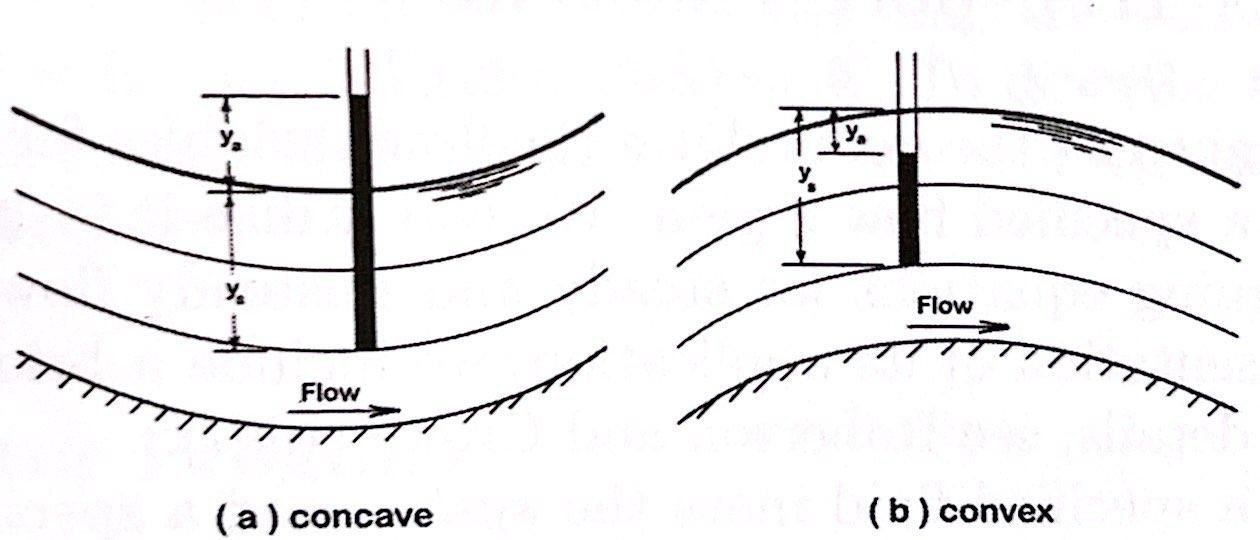
\includegraphics[width=0.9\textwidth]{fig8.jpeg}
\caption{Fuerzas actuantes sobre un elemento de flujo curvil\'ineo (tomado de \cite{Chau}).}
\label{fig8}
\end{figure}

Si la curvatura de las lineas de flujo es $r$ y la velocidad en un punto es  $V$, tenemos que la $\text{aceleración centrifuga}= \frac{V^2}{r}$ y la $\text{fuerza centrifuga}= \rho y_s dA \frac{V^2}{r}$ donde $y_s$ es la altura hidroest\'atica, $y_a$ es la corrección de la altura de presi\'on por curvatura y $h = y_s \pm y_a$ es la altura piezom\'etrica. En el caso de flujo convexo las fuerzas actúan hacia arriba y la altura piezom\'etria $h = y_s-y_a$; en el caso del flujo cóncavo, la altura piezom\'etrica es $h = y_s+y_a$. $y_a$ se calcula a partir de la fuerza centrifuga:
$$
y_a = \frac{1}{g}y_s \frac{V^2}{r}
$$

La altura piezom\'etrica se calcula entonces como:
$$
h = y_s \left( 1 \pm \frac{1}{g} \frac{V^2}{r} \right)
$$

Note que $h$ representa la cabeza de energ\'ia de presi\'on. 

\begin{alg}{Calculo de los coeficientes de energ\'ia y de cantidad de movimiento}{alg1}
\begin{enumerate}
\item Leer la siguiente informaci\'on: $l$, $xs$, $ys$ y $Vs$. Note que $xs$ y $ys$ son dos vectores con las coordenadas $x$ y $y$ respectivamente para un numero $m$ de puntos que conforman la seci\'on transversal. $Vs$ es un vector de velocidades medias de $m-1$ segmentos que conforman la secci\'on.
\item Con base en las coordenadas datas ($xs$ y $ys$), interpolar un nuevo conjunto de puntos para el nivel $l$.   
\item Calcular el \'area de cada segmento de \'area $A_i$, con base en el nuevo conjunto de puntos ($xs$ y $ys$).
\item Con base en los valores de $A_i$ y de $Vs$, calcular el coeficiente de energ\'ia ($\alpha$) con la ecuaci\'on~\ref{alp3} y el coeficiente de cantidad de movimiento ($\beta$) usando la ecuaci\'on~\ref{bet3}.
\item Imprimir: Coeficiente de energ\'ia ($\alpha$) y el coeficiente de cantidad de movimiento ($\beta$). 
\end{enumerate}
\end{alg}

\begin{eje}{}{eje1}
    Para el canal trapezoidal de la figura, cuyas velocidades en $m/s$ han sido medidas en los puntos medios de las secciones, calcular el coeficiente de energ\'ia y de cantidad de movimiento.
    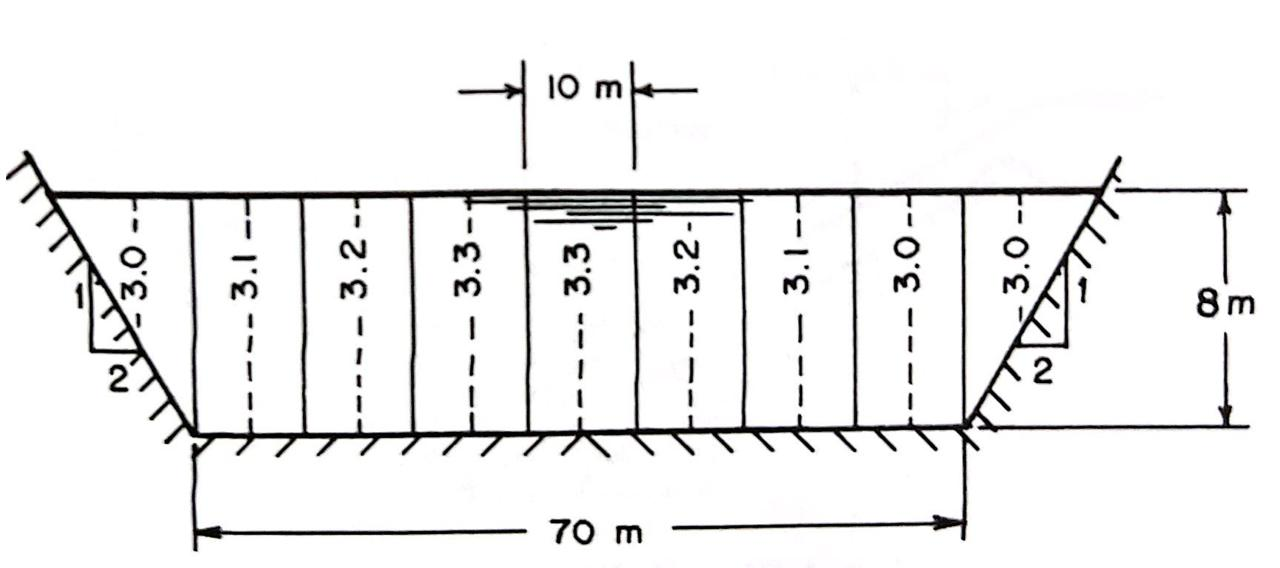
\includegraphics[width=8cm]{fig118.jpeg} %Fig 1.18 from Chau
\end{eje}


%%%%%
\section{Conservaci\'on de la energ\'ia}% From VChow
La energ\'ia total del flujo ($H$) en un punto $A$ de una secci\'on transversal de canal en unidades de fuerza por unidades de longitud sobre unidades de fuerza, con respecto a un nivel de referencia (ver figura~\ref{fig9}), est\'a dada por ecuaci\'on:

% VChow fig 3.1
\begin{figure}[h]
\centering
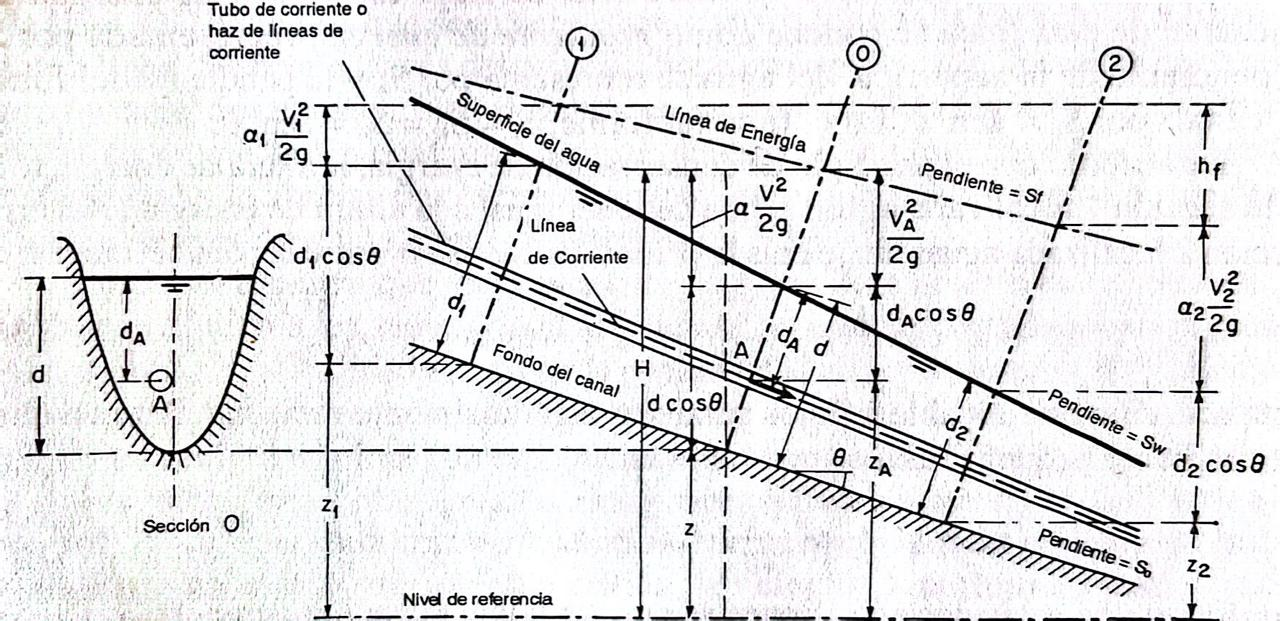
\includegraphics[width=0.9\textwidth]{fig31.jpeg}
\caption{Energ\'ia en un flujo gradualmente variado en un canal a superficie libre (tomado de \cite{VChow}).}
\label{fig9}
\end{figure}

\begin{equation}
H = z_{A} + d_{A} \cos \theta + \frac{U_A^2}{2g} 
\label{ene1}
\end{equation}

donde $z_A$ es el nivel de un elemento de fluido $A$ contenido en una l\'inea de corriente con respecto a un nivel de referencia, $d_A$ es la profundidad del elemento de fluido $A$ medida desde la superficie libre, $\theta$ es el \'angulo de inclinaci\'on del canal y $V_A$ es la velocidad de flujo en el punto $A$. Para efectos pr\'acticos, la distribuci\'on de velocidades en la secci\'on se considera uniforme, por lo que el termino de la cabeza de energ\'ia cin\'etica de la ecuaci\'on~\ref{ene1} se corrige utilizando el coeficiente de energ\'ia ($\alpha$) para tener en cuenta la distribuci\'on no uniforme de velocidades en la secci\'on. Para una secci\'on cualquiera, tenemos:

\begin{equation}
\color{red}\boxed{\color{black} H = z + d \cos \theta + \alpha\frac{V^2}{2g} }
\label{ene2}
\end{equation}

donde $z$ es el nivel del fondo del canal y representa la \emph{cabeza de energ\'ia potencial} del flujo, $d$ es la profundidad de la secci\'on medida perpendicular desde la superficie hasta el fondo del canal y representa la \emph{cabeza de energ\'ia de presi\'on} y $V$ es la velocidad media en la secci\'on. El t\'ermino $\alpha \frac{V^2}{2g}$ representa la \emph{cabeza de energ\'ia cin\'etica} corregida del flujo. Si $\theta \approx 0$, el termino $d \cos \theta \approx d = y$, donde $y$ es la profundidad del flujo. 

Analizando la figura~\ref{fig9} y teniendo en cuenta que la ecuacio\'on~\ref{ene2} representa la energ\'ia en una secci\'on del canal, la pendiente de la l\'inea energ\'ia conocida como \emph{gradiente de energ\'ia} se representa como $S_f=\frac{h_f}{L}$ donde $h_f$ es la p\'erdida de energ\'ia entre dos secciones y $L$ es la distancia horizontal entre las secciones. Para el caso de \emph{flujo uniforme} la pendiente de la l\'inea de energ\'ia ($S_w$) y la pendiente del fondo del canal ($S_o \approx \sin \theta$) son iguales al gradiente de energ\'ia: $S_f = S_w = S_o = \sin \theta$. Note que $\tan \theta \approx \sin \theta$ cuando $\theta \approx 0$. 

De acuerdo con el principio de conservaci\'on de energ\'ia, la energ\'ia total entre dos secciones 1 y 2, se representa como:

\begin{equation}
z_1 + d_1 \cos \theta + \alpha_1 \frac{V_1^2}{2g} = z_2 + d_2 \cos \theta + \alpha_2 \frac{V_2^2}{2g} + h_{f}
\label{ene3}
\end{equation}

Para un canal con pendiente peque\~na, se tiene:

\begin{equation}
 z_1 + d_1 + \alpha_1 \frac{V_1^2}{2g} = z_2 + d_2 + \alpha_2 \frac{V_2^2}{2g} + h_{f}
\label{ene4}
\end{equation}

Si $\alpha_1 \approx \alpha_2 \approx 1$ y $h_f \approx 0$, la ecuaci\'on~\ref{ene4} se convierte en la \emph{ecuaci\'on de Bernoulli}:

\begin{equation}
\color{red}\boxed{\color{black} z_1 + d_1 + \frac{V_1^2}{2g} = z_2 + d_2 + \frac{V_2^2}{2g} = \text{constante}}
\label{ene5}
\end{equation}

\subsection{Energ\'ia espec\'ifica}
La \emph{energ\'ia espec\'ifica} en la secci\'on de un canal es la energ\'ia por unidad de fuerza con respecto al fondo del canal($z=0$). A partir de la ecuaci\'on~\ref{ene2}, se tiene:

\begin{equation}
\color{red}\boxed{\color{black} E =   d\cos \theta + \alpha\frac{V^2}{2g}}
\label{ene6}
\end{equation}

Cuando $\theta \approx 0$ y $\alpha = 1$, la ecuaci\'on anterior queda:
 
\begin{equation}
\color{red}\boxed{\color{black} E =   y  + \frac{V^2}{2g} = y + \frac{Q^2}{2g A^2 }}
\label{ene7}
\end{equation}

donde $Q$ es el caudal medio que pasa a trav\'es de la secci\'on del canal y $A$ es el \'area transversal de la secci\'on del canal. La ecuaci\'on~\ref{ene7} muestra que la energ\'ia espec\'ifica en la secci\'on de un canal es igual a la profundidad de flujo m\'as la cabeza de energ\'ia cin\'etica del flujo. Note que si $Q$ es conocido, la ecuaci\'on~\ref{ene7} se convierte en  una  funci\'on $y$.

Graficando la ecuaci\'on~\ref{ene7} se tiene la \emph{curva de energ\'ia especifica} (ver figura~\ref{fig10}), en donde las abscisas est\'an representadas por $E$ y las ordenadas por $y$.
% VChow fig 3.2
\begin{figure}[h]
\centering
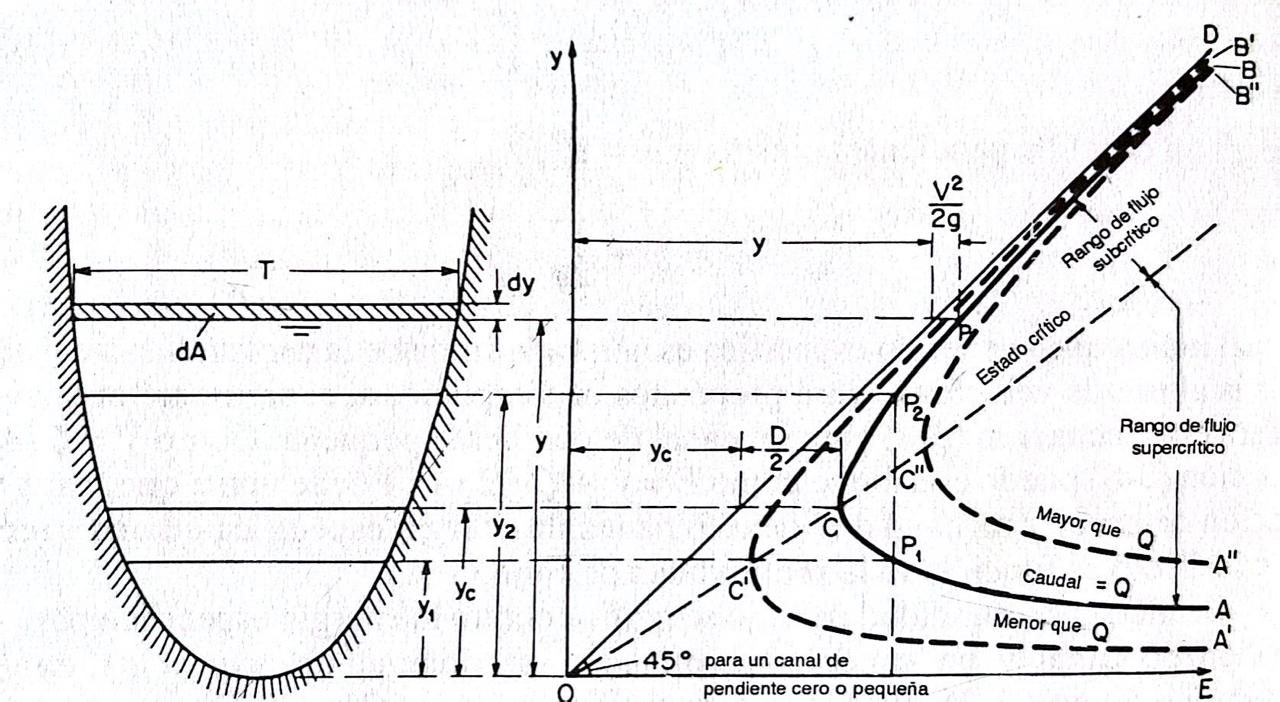
\includegraphics[width=0.9\textwidth]{fig32.jpeg}
\caption{Curva de energ\'ia espec\'ifica (tomado de \cite{VChow}).}
\label{fig10}
\end{figure}

Esta curva tiene dos asíntotas: $y=0$ y $y=E$ (curva OD) para los cuales $E$ tiende a infinito. Note que para canales horizontales, la curva OD forma un angulo de 45$^o$. Para canales de alta pendiente, la asíntota es $y=E=d \cos \theta$, por lo que el angulo es igual a $\cos \theta$. La curva ademas evidencia lo siguiente:
\begin{itemize}
\item Para un valor de $E$ existen dos posibles valores de $y$: $y_1$ y $y_2$. Est\'an dos profundidades son conocidas como las \emph{profundidades alternas}.
\item El valor m\'inimo de la energ\'ia $E$ ocurre en el punto $C$. La profundidad all\'i es una sola y se conoce como la \emph{profundidad cr\'itica} ($y_c$). El flujo para $y_c$ tiene una \emph{velocidad cr\'itica} ($V_c$). 
\item Cuando $y > y_c$, la velocidad del flujo ($V$) es mayor que $V_c$ y por lo tanto el flujo es \emph{supercr\'itico}. Cuando $y < y_c$, la velocidad del flujo ($V$) es menor que $V_c$ y por lo tanto el flujo es \emph{subcr\'itico}.
\item Si el caudal aumenta en la ecuaci\'on~\ref{ene7}, la curva de energ\'ia espec\'ifica se desplaza hacia la derecha, si disminuye se desplaza hacia la izquierda. 
\end{itemize}

\subsection{Flujo cr\'itico}
El \emph{flujo critico} se define como aquel flujo para el cual el n\'umero de Froude ($F_r$) es igual a 1. Tambi\'en se puede definir como el flujo para el cual la energ\'ia espec\'ififa es minima. Teniendo en cuenta que $E=f(y)$, la energ\'ia espec\'ifica minima o critica, puede encontrar derivando la ecuaci\'on~\ref{ene7} con respecto a $y$:
$$
\frac{dE}{dy} = 1 - \frac{Q^2}{gA^3} \frac{dA}{dy} = 1 - \frac{V^2}{gA} \frac{dA}{dy}
$$
donde $\frac{dA}{dy} \approx T$, donde $T$ es el ancho superficial de la secci\'on. Teniendo en cuenta que $A/T$ es conocida como la profundidad hidr\'aulica, tenemos:
$$
\frac{dE}{dy} = 1 -  \frac{V^2 T}{gA} = 1 -  \frac{V^2}{gD} 
$$
Si la energ\'ia es m\'inima cuando  $\frac{dE}{dy}=0$, la expresi\'on anterior queda:

\begin{equation}
\frac{V^2}{2g} = \frac{D}{2} 
\label{ene8}
\end{equation}

Esta ecuaci\'on indica que la cabeza de energ\'ia cinem\'atica es igual a la mitad de la profundidad hidr\'aulica para flujo cr\'itico. La ecuaci\'on anterior tambi\'en se puede expresar como $\frac{V}{\sqrt{gD}}=1$ el cual es ecuaci\'on de $F_r$ para flujo cr\'itico. La ecuaci\'on~\ref{ene8} se aplica para canales con pendiente baja y $\alpha = 1$. Para canales con pendiente alta y valores de $\alpha \ne 1$, la ecuaci\'on~\ref{ene8} se convierte:

\begin{equation}
\alpha \frac{V^2}{2g} = \frac{\cos \theta D}{2} 
\label{ene9}
\end{equation}

\subsection{Fen\'omenos locales}
Los fen\'omenos locales ocurren frecuentemente en canales cuando hay cambios de r\'egimen (de subcr\'itico a supercr\'itico o viceversa) en distancias. Existen dos tipos principales:
\begin{itemize}
\item \emph{Ca\'ida hidr\'aulica}: Se presenta cuando hay un cambio brusco de la pendiente del fondo del canal lo cual hace que el flujo pase de ser subcr\'itico a supercr\'itico en una secci\'on de transici\'on en donde se presenta  la profundidad cr\'itica. 
\item \emph{Ca\'ida libre}: La ca\'ida libre se presenta cuando el fondo del canal cambia abruptamente, como por ejemplo, en la descarga libre de un canal a un lago. En la ca\'ida libre, el flujo va de flujo subcr\'itico antes de la ca\'ida alcanzando su energ\'ia m\'inima justo en la secci\'on de la descarga. Sin embargo, an\'alisis experimentales han encontrado que la secci\'on de energ\'ia cr\'itica no es exactamente en la secci\'on de la descarga debido a la curvatura de la l\'amina de agua por lo que para pendientes pequeñas $y_c = 1.4 y_o$, donde $y_o$ es la profundidad en el borde y $y_c$ se localiza entre 3 y 4 $y_c$ aguas arriba del borde del canal.
\item \emph{Resalto hidr\'aulico}: Se presenta cuando existe un aumento r\'apido de la l\'amina de agua que puede ser causado aguas abajo del flujo bajo una compuerta  en un canal horizontal, o al final de un vertedero cuando la pendiente alta se vuelve casi horizontal. 
\end{itemize}
Es importante señalar que la descripci\'on de la curva de energ\'ia espec\'ifica se ha presentado para canales prism\'aticos. En el caso de canales naturales en donde las secciones cambia constantemente a lo largo del canal, la curva de energ\'ia espec\'ifica varia de igual manera as\'i como la profundidad cr\'itica en cada secci\'on. El c\'alculo de la curva para canales naturales se hace num\'ericamente a partir de las ecuaciones descritas anteriormente. 

\begin{eje}{}{eje2}
  For all natural number $n$ it holds:
\end{eje}

%%%%%
\section{Conservaci\'on de la cantidad de movimiento}% From VChow
La cantidad de movimiento que pasa a tr\'avez de una secci\'on de un canal por unidad de tiempo se expresa como $\beta\frac{ \gamma Q V}{g}$. De acuerdo con la \emph{segunda ley de Newton}, para un canal de pendiente alta, el cambio de la cantidad de movimiento por unidad de tiempo entre dos secciones de canal (1 y 2) en la direcci\'on del flujo es igual a las fuerzas externas actuantes sobre el volumen de control conformado por las dos secciones (ver figura~\ref{fig11}). La siguiente ecuaci\'on se conoce como la ecuaci\'on de conservaci\'on de la cantidad de movimiento:

\begin{equation}
\frac{\gamma}{g}\left(\beta_2 Q_2 V_2 - \beta_1 Q_1 V_1 \right) = A_1 P_1 - A_2 P_2 + w \sin \theta - F_f
\label{ene10}
\end{equation}

% VChow fig 3.7
\begin{figure}[h]
\centering
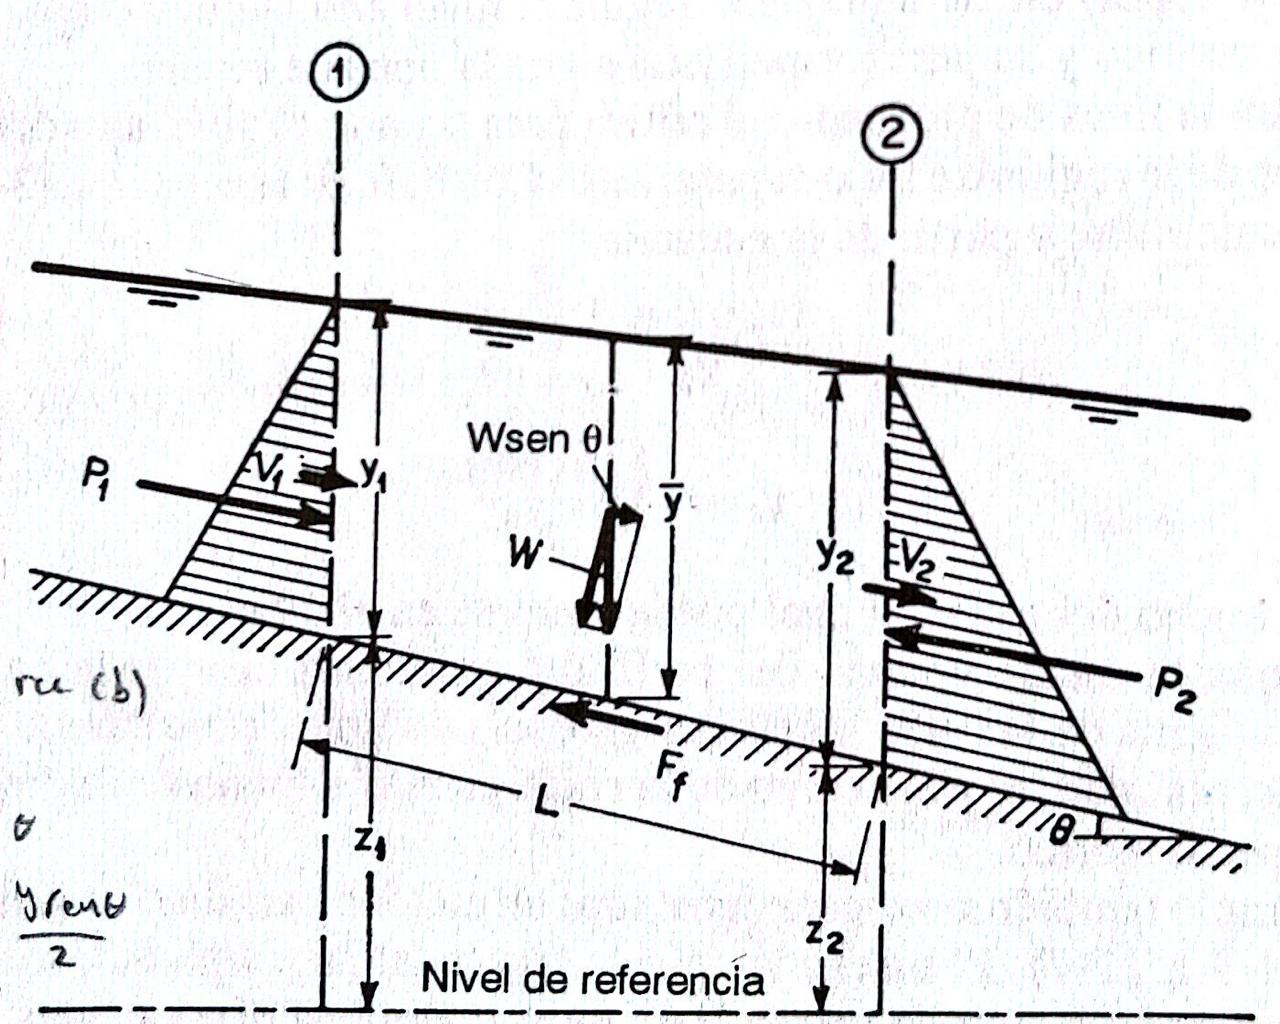
\includegraphics[width=0.9\textwidth]{fig37.jpeg}
\caption{Aplicaci\'on del principio  cantidad de movimiento (tomado de \cite{VChow}).}
\label{fig11}
\end{figure}


donde $\gamma$ es el peso especifico del liquido, $P=\gamma \bar{z}$, es la presi\'on resultante sobre la secci\'on donde $\bar{z}$ es la  profundidad del centroide del \'area mojada $A$, $w$ es el peso del l\'iquido entre las secciones 1 y 2, y $F_f$ es la fuerza de fricci\'on que se opone al flujo y que act\'ua a lo largo de la superficie de contacto entre el flujo y el canal; esta fuerza nada tiene que ver con las p\'erdidas de energ\'ia dentro del elemento de fluido. Para flujos gradualmente variados, los valores de $P$ representan la presi\'on hidroest\'atica. Sin embargo, para el caso de flujo r\'apidamente variado o curvil\'ineo, la presi\'on no es hidroest\'atica y dichos valores de $P$ deben corregirse a trav\'es de un \emph{coeficiente de distribuci\'on de presiones} o tambi\'en conocido como \emph{coeficiente de fuerza} $\nu$. Este coeficiente se calcula como: 

$$
\nu = \frac{1}{A\bar{z}} \int_0^A h dA = 1 + \frac{1}{A\bar{z}} \int_0^A y_a dA
$$

donde $h$ es la profundidad del elemento $dA$ y $y_a$ es la correci\'on de la altura piezom\'etrica $y_a=\frac{y_s V^2}{gr}$. De acuerdo con la ecuaci\'on anterior, se puede ver que $\nu < 1$ cuando la curvatura es convexa, $\nu > 1$ cuando la curvatura es c\'oncava e igual a 1 para flujo paralelo o gradualmente variado. 

Para el caso se flujo gradualmente variado con una pendiente baja ($\nu \approx 1$) la ecuaci\'on~\ref{ene10} se convierte en:

\begin{equation}
\color{red}\boxed{\color{black} \frac{\gamma}{g}\left(\beta_2 Q_2 V_2 - \beta_1 Q_1 V_1 \right) = \gamma \left( A_1 \bar{z_1} - A_2 \bar{z_2} \right) - w \sin \theta - F_f}
\label{ene11}
\end{equation}

La ecuaci\'on~\ref{ene11} representa la ecuaci\'on general de la conservaci\'on de cantidad de movimiento. 
\subsection{Fuerza especifica}
Para el caso de un canal prism\'atico casi horizontal ($\theta \approx 0$) y de secci\'on de material suave ($F_f \approx 0$) en donde la distribuci\'on de las velocidades es uniforme ($\beta \approx 0$), la ecuaci\'on~\ref{ene11} queda:

\begin{equation}
Q_2 V_2 - Q_1 V_1 = g \left( A_1 \bar{z_1} - A_2 \bar{z_2} \right)
\label{ene12}
\end{equation}

De la ecuac\'on de continuidad $Q_1 = V_1 A_1 = Q_2 = V_2 A_2 = Q$, reemplazando en la ecuaci\'on anterior y organizando los t\'erminos:

\begin{equation}
\color{red}\boxed{\color{black}\frac{Q^2}{g A_1} + \bar{z_1}A_1 = \frac{Q^2}{g A_2} + \bar{z_2}A_2 }
\label{ene13}
\end{equation}

De la ecuaci\'on~\ref{ene13}, se puede determinar que los dos lados de la igualdad son iguales; cualquier t\'ermino se denomina \emph{fuerza especifica}

\begin{equation}
\color{red}\boxed{\color{black} F_s = \frac{Q^2}{g A} + \bar{z}A  }
\label{ene14}
\end{equation}

La ecuaci\'on~\ref{ene14} esta en unidades de fuerza por unidad de peso espec\'ifico. La ecuaci\'on~\ref{ene14} se puede expresar como $F_{s_1} = F_{s_2}$ lo cual indica que la fuerza espec\'ifica en dos secciones de un canal es la misma siempre y cuando la fuerza externa ejercida por las paredes del canal sobre el flujo sea despreciable. Para el caso de un canal rectangular ancho de base $b$, $\bar{z} = \frac{y}{2}$ y $A=by$, la ecuaci\'on~\ref{ene14} se vuelve:

\begin{equation}
\color{red}\boxed{\color{black} F_s = \frac{Q^2}{g by} + \frac{by^2}{2} }
\label{ene15}
\end{equation}

%%%%%
\section{Casos de aplicaci\'on de la conservaci\'on de la energ\'ia y del momento lineal}
\subsection{Trancisi\'on en un canal}
Una transici\'on en un canal es un cambio subido o gradual en el ancho del canal, en el fondo del canal o en ambos (ver figura~\ref{fig12}). Usualmente, estas transiciones se diseñan de tal manera que las p\'erdidas de energ\'ia son despreciables. Es por esto que la ecuaci\'on de conservaci\'on de la energ\'ia es la m\'as apropiada para el an\'alisis. 

% Chau fig 2.8
\begin{figure}[h]
\centering
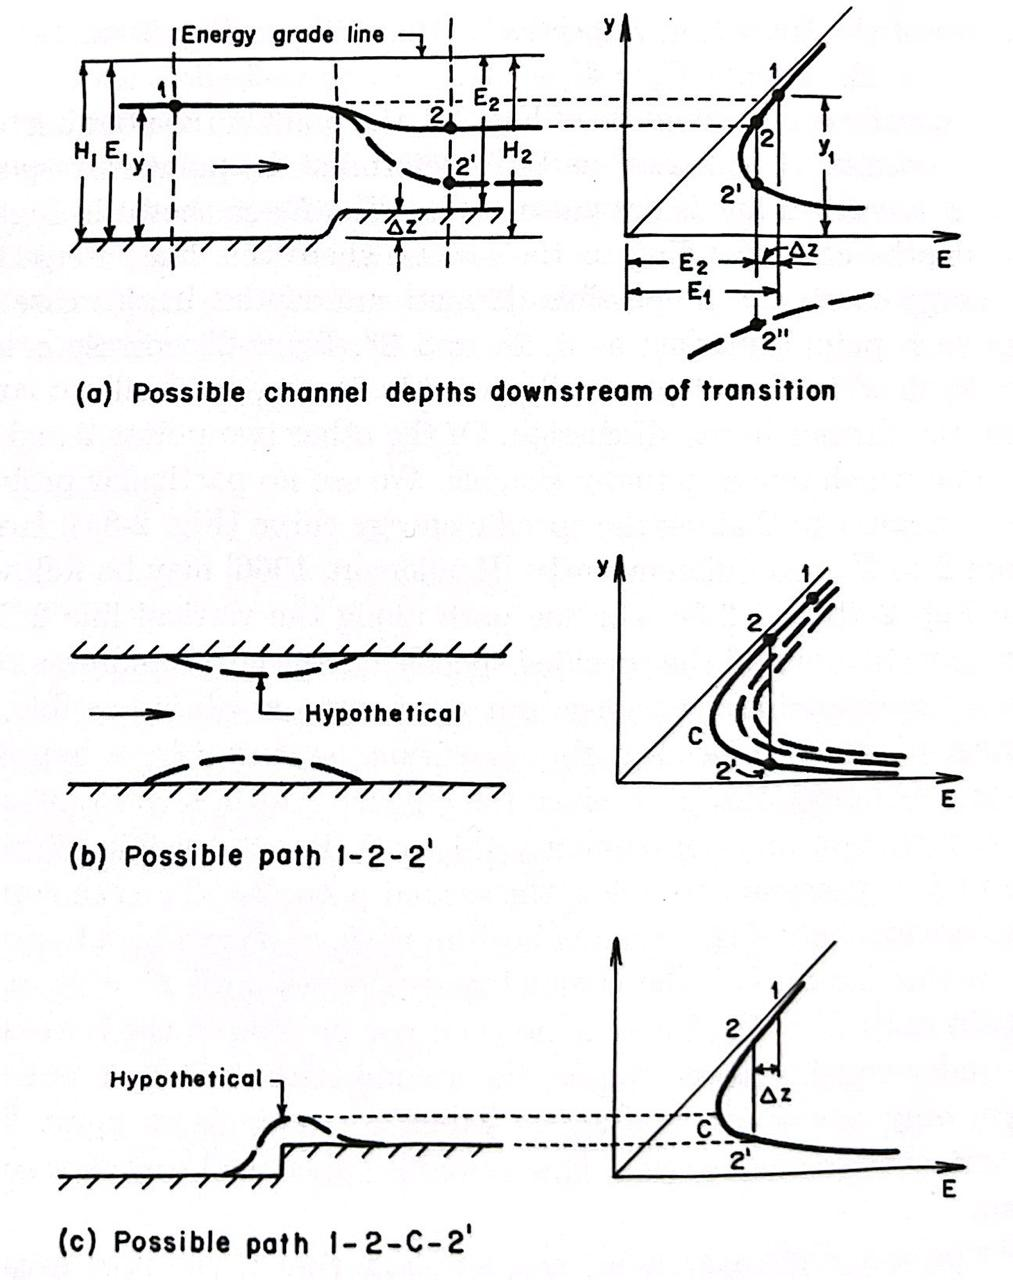
\includegraphics[width=0.9\textwidth]{fig28.jpeg}
\caption{Transici\'on en un canal de ancho constante (tomado de \cite{Chau}).}
\label{fig12}
\end{figure}

Si se analiza el caso de un canal rectangular de ancho constante $b$ con un escal\'on en el fondo (ver figura~\ref{fig12}), se desea obtener, a partir de una profundidad y velocidad conocida aguas arriba, ¿que sucede con la profundidad aguas abajo de la transici\'on?. Teniendo en cuanta que las p\'erdidas en la transici\'on son despreciables la cabeza antes y despu\'es son las mismas $H_1 = H_2$. Sin embargo, analizando la energ\'ia especifica en ambas secciones, se tiene que $E_1 = H_1$ y $E_2 = H_2-\Delta z$, por lo que $E_2 = E_1 - \Delta z$. Para saber cual es la profundidad aguas abajo de la transici\'on es necesario analizar la curva de energ\'ia espec\'ifica (figura~\ref{fig12}a). Si la profundidad aguas arriba es $y_1$ esta necesariamente se debe desplazas hacia la izquierda teniendo en cuenta $\Delta z$. Al desplazarse a la izquierda la profundidad $y_2$ puede ser para los puntos 2, 2' o 2". El punto 2" implica una profundidad negativa por lo que se descarta. No habr\'ia problema de ir de 1 a 2. Sin embargo, para ir de 1 a 2', ser\'ia necesario que la curva de caudal espec\'ifico se desplazara a la derecha en el evento en que hubiera en la transici\'on una reducci\'on del ancho que aumentara el caudal unitario ($Q/b$) de tal manera que el flujo pasara por $y_c$ en alg\'un punto de la reducci\'on y luego pasara a 2' (ver figura~\ref{fig12}b). Sin embargo, esto no es posible porque la secci\'on del canal es constante. La otra posibilidad es que el escalón fuera lo suficientemente alto para que la p\'erdida de energ\'ia especifica fuera tal que la energ\'ia en la cima del escal\'on fuera $E_c$ (ver figura~\ref{fig12}c). Sin embargo, esto tampoco es posible por que la p\'erdida por $\Delta z$ no es tan grande para que esto suceda. Finalmente, la profundidad cambiar\'ia de 1 a 2 y quiere decir que el r\'egimen de flujo permanece subcr\'itico aguas abajo. En el caso en el que el flujo fuera supercr\'itico aguas arriba, habr\'ia la posibilidad de ir de 1 a 2 o 2' (ver figura~\ref{fig13}). Sin embargo, para $\Delta z$ $y$ iría de 1 a 2 y flujo seguir\'ia siendo supercr\'itico. 

% Chau fig 2.9
\begin{figure}[h]
\centering
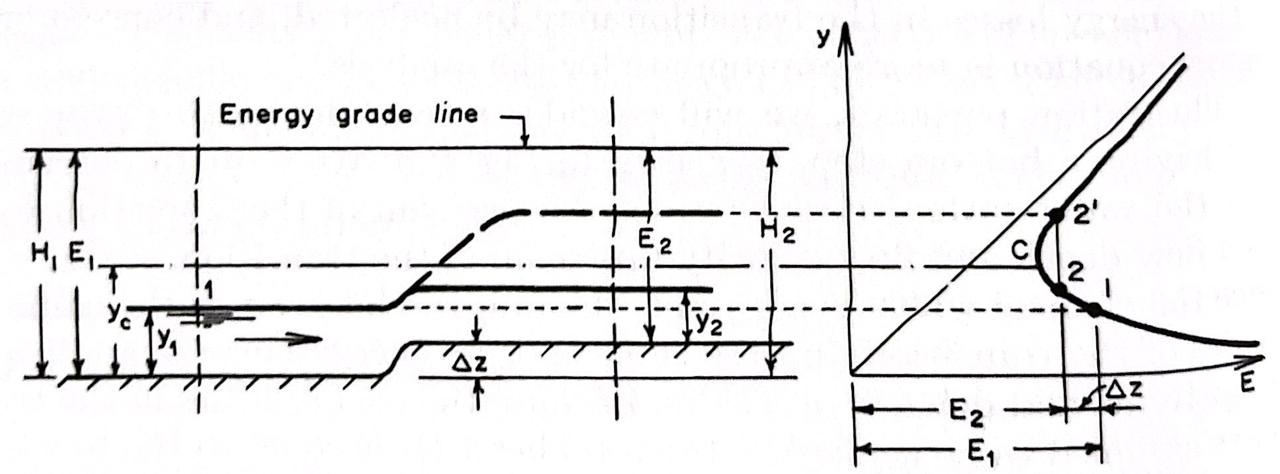
\includegraphics[width=0.8\textwidth]{fig29.jpeg}
\caption{Transici\'on con flujo supercritico aguas arriba (tomado de \cite{Chau}).}
\label{fig13}
\end{figure}

De acuerdo con los dos casos presentados en las figuras~\ref{fig12} y ~\ref{fig13}, si el flujo es subcr\'itico aguas arriba, aguas abajo este permanece igual pero con una reducci\'on en $y$. En el caso de tener un flujo supercr\'itico aguas arriba, aguas abajo el flujo sigue siendo el mismo pero con un aumento de $y$.

Para determinar cual es la variaci\'on de $y$ con respecto a una variaci\'on del fondo del canal $z$, se analiza la ecuaci\'on de la cabeza de energ\'ia para un flujo paralelo o gradualmente variado cuya presi\'on es hidroest\'atica y con distribuci\'on de velocidad uniforme. Se tiene:

\begin{equation}
H = z + y + \frac{Q^2}{2g A^2}
\label{ene16}
\end{equation}

Derivando la ecuaci\'on~\ref{ene16} con respecto a $x$, teniendo en cuenta que $x$ aumenta positivamente hacia aguas abajo, se tiene:

\begin{equation}
\frac{dH}{dx} = \frac{dz}{dx} + \frac{dy}{dx} + \frac{Q^2}{2g}\frac{d}{dx}\left( \frac{1}{A^2} \right)
\label{ene17}
\end{equation}

como:
$$
\frac{d}{dx}\left( \frac{1}{A^2} \right) = \frac{-2}{A^3}\frac{dA}{dx}
$$
por \emph{regla de la cadena}:

$$
\frac{dA}{dx} = \frac{dA}{dy}\frac{dy}{dx}
$$

para un cambio pequeño en $y$, $\Delta y$, tenemos que $\Delta A \approx T \Delta y$, donde $T$ es el ancho en la superficie libre. Aplicando l\'imites, se tiene que $dA = Tdy$ y:
$$
\frac{dA}{dx} = T \frac{dy}{dx}
$$

Adicionalmente, de la defici\'on de numero de Froude, se tiene:

\begin{equation}
F_r^2 = \frac{V^2}{g A/T} = \frac{Q^2 T}{g A^3}
\label{ene18}
\end{equation}

Reemplazando en la ecuaci\'on~\ref{ene17}, se tiene que:

\begin{equation}
\frac{dH}{dx} = \frac{dz}{dx} + \left( 1- F_r^2 \right)\frac{dy}{dx}
\label{ene19}
\end{equation}

Como no se consideran p\'erdidas de energ\'ia, $\frac{dH}{dx} = 0$, la ecuaci\'on~\ref{ene19} se convierte:

\begin{equation}
\color{red}\boxed{\color{black} \frac{dz}{dx} = \left( F_r^2 - 1 \right)\frac{dy}{dx} }
\label{ene20}
\end{equation}

La ecuaci\'on~\ref{ene20} relaciona las variaciones del fondo del canal con la variaci\'on de la profundidad de agua. Si hay un aumento del fondo del canal, $\frac{dz}{dx} > 0$, por lo que el t\'ermino derecho de la ecuaci\'on~\ref{ene20} debe ser positivo y para esto $\left( F_r^2 - 1 \right)$ y  $\frac{dy}{dx}$ son ambos positivos o ambos negativos. Si ambos son positivos, esto implica que haya un aumento de profundidad ($y_2 > y_1$) y que $F_r^2 > 1$ para lo cual $F_r > 1$ (flujo supercr\'itico). Si ambos son negativos, esto implica una disminuci\'on de la profundidad ($y_2 < y_1$) y que $F_r^2 < 1$ para lo cual $F_r < 1$ (flujo subcr\'itico). Un an\'alisis similar es posible sin en lugar de tener un aumento del fondo se tiene una ca\'ida del fondo. 
 
% Eje 2-1 Chau
\begin{eje}{}{eje3}
  For all natural number $n$ it holds:
\end{eje}


\subsection{Resalto hidr\'aulico}
Un \emph{resalto hidr\'aulico} es un fen\'omeno que se forma en un canal cuando existe un cambio de flujo supercr\'itico a subcr\'itico. Se presenta entonces una discontinuidad muy fuerte en la l\'amina de agua en donde adem\'as, debido a la turbulencia que se genera dentro del resalto hidr\'aulico, existe una p\'erdida de energ\'ia considerable. Es por esto que los resaltos hidr\'aulicos se forman para mezclar sustancias en el flujo, para disipar energ\'ia en estructuras hidr\'aulicas y para oxigenar flujos de agua. Las profundidades de la l\'amina de agua justo antes y despu\'es del resalto se denominan \emph{alturas conjugadas} (ver figura~\ref{fig14}). 

% Chau fig 2.11
\begin{figure}[h]
\centering
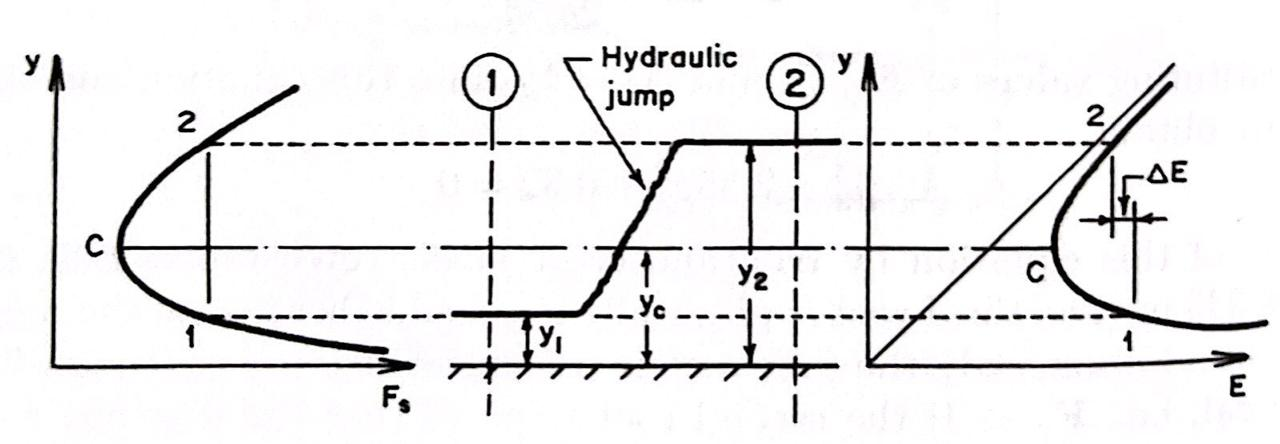
\includegraphics[width=0.8\textwidth]{fig211.jpeg}
\caption{Transici\'on con flujo supercr\'itico aguas arriba (tomado de \cite{Chau}).}
\label{fig14}
\end{figure}

Un resalto hidr\'aulica posee las siguientes caracter\'isticas:
\begin{enumerate}
\item Existen perdidas de energ\'ia en el resalto hidr\'aulico debido a la turbulencia que se genera dentro del flujo, por lo que $\Delta H = H_1 - H_2 > 0$.
\item Teniendo en cuenta que las fuerzas de fricci\'on que ejercen las paredes sobre el flujo son despreciables, y que para canales con pendiente baja ($\theta \approx 0$) la componente del peso en la direcci\'on del flujo es cero, las fuerzas especificas antes y después del resalto son iguales $F_{s_1} = F_{s_2}$. 
\item Se cumple la ecuaci\'on de continuidad, $Q_1 = V_1 A_1 = Q_2 = V_2 A_2$.
\end{enumerate}

Supongamos que tenemos un canal horizontal de secci\'on rectangular de ancho $b$ cuya distribuci\'on de velocidades en la secci\'on es uniforme. Para este caso es posible encontrar una expresi\'on que relacione las alturas conjugadas a partir del supuesto $F_{s_1} = F_{s_2}$. Partiendo de la ecuaci\'on~\ref{ene11} tenemos:

%Para esto es necesario saber que existen  perdidas de energia en el resalto, sin embargo no se tiene para lo cual no se tiene un expresion. Si analizamos las fuerzas actuantes antes y despues del resalto, se puede afirmar que las fuerzas debido a la fricci\'on son despreciables con relacion a por ejemplo las fuerzas hidroestaticas. La componente del peso es tambien cero. Aplicando la ecuacion~\ref{ene11} nos queda entonces:
$$
\frac{Q^2}{g A_1} + \bar{z_1}A_1 = \frac{Q^2}{g A_2} + \bar{z_2}A_2 
$$

reorganizando los t\'erminos, se tiene:

$$
\frac{Q^2}{g}\left( \frac{1}{A_1} - \frac{1}{A_2} \right) = \bar{z_2}A_2 - \bar{z_1}A_1 
$$

Si $A=by$ y $\bar{z}=\frac{y}{2}$, y reorganizando t\'erminos, se tiene:

$$
\frac{Q^2}{bg}\left( \frac{y_2 - y_1 }{y_2 y_1}\right) = \frac{b}{2}\left( y_2^2 - y_1^2 \right)
$$

Simplificando, se tiene:

$$
\frac{2 Q^2}{b^2 g}\left( \frac{1}{y_2 y_1}\right) = y_2 + y_1
$$

De la ecuaci\'on de continuidad para la secci\'on 1, $Q=A_1 V_1 = by_1 V_1$, reemplazando y simplificando:

$$
\frac{2 V_1^2 y_1}{g y_2} = y_2 + y_1
$$

Dividiendo a ambos lados $y_1^2$, simplificando y reagrupando:

$$
\frac{V_1^2}{g y_1} = \frac{y_2}{2 y_1}\left( y_2 + y_1 \right)
$$

De la definici\'on de n\'umero de Froude para la secci\'on 1, $F_{r_1}^2 =\frac{V_1^2}{g y_1}$ y reorganizando los t\'erminos, se tiene:

$$
2 F_{r_1}^2 = \left( \frac{y_2}{y_1} \right)^2 + \frac{y_2}{y_1}
$$

Reorganizando los t\'erminos, tenemos:

$$
\left( \frac{y_2}{y_1} \right)^2 + \frac{y_2}{y_1} - 2 F_{r_1}^2 =0
$$
La ecuaci\'on anterior tiene la forma de una ecuaci\'on cuadr\'atica $ax^2 + bx + c =0 $, donde $x= \frac{y_2}{y_1}$. Para encontrar la soluci\'on se aplica la ecuaci\'on $x = \frac{-b \pm \sqrt{b^2-4ac}}{2a}$, donde $a=1$, $b=1$ y $c=2F_{r_1}^2$, lo cual queda:

\begin{equation}
\color{red}\boxed{\color{black} \left( \frac{y_2}{y_1} \right) = \frac{1}{2} \left( -1 + \sqrt{1 + 8 F_{r_1}^2} \right)}
\label{ene21}
\end{equation}

Note que se toma la raíz positiva para obtener las soluciones de la ecuaci\'on, de no ser as\'i. $\frac{y_2}{y_1} < 0$ lo cual no es posible f\'isicamente. Si en lugar se aplica la ecuaci\'on de continuidad para la secci\'on 2 $Q=A_2 V_2 = by_2 V_2$ y la definici\'on de n\'umero de Froude para esta secci\'on, se tiene una ecuaci\'on similar a la ecuaci\'on~\ref{ene21}:

\begin{equation}
\color{red}\boxed{\color{black} \left( \frac{y_1}{y_2} \right) = \frac{1}{2} \left( -1 + \sqrt{1 + 8 F_{r_2}^2} \right)}
\label{ene22}
\end{equation}

Las ecuaciones~\ref{ene21} y ~\ref{ene22} indican que es posible obtener la profundidad de una secci\'on si se conoce la profundidad y la velocidad de la otra secci\'on. Al conocerse $y_1$, $V_1$, $y_2$ y $V_2$, es posible luego conocer las p\'erdidas de energ\'ia en el resalto.

De acuerdo con an\'alisis experimentales y con base en las ecuaciones anteriores, se describen algunas propiedades del resalto hidr\'aulico:
\begin{itemize}
\item \textbf{Relaci\'on de las profundidade conjugadas}: Analizando la ecuaci\'on~\ref{ene21}, la relaci\'on de las profundidades conjugadas $y_r = \frac{y_2}{y_1}$ se convierte en:
$$
y_r = \sqrt{2} F_{r_1} - \frac{1}{2}
$$
cuando $F_{r_1} > 2$ ya que el valor de $\sqrt{1+8F_{r_1}^2} \approx \sqrt{2} F_{r_1}$. Esto indica una relaci\'on lineal entre $y_r$ y $F_{r_1}$.

\item \textbf{Longitud del resalto}: La longitud del resalto $L$ es importante para el diseño de tanques disipadores de energía o de mezcla. Esta longitud difiere de la longitud de la turbulencia $L_r$ que es mas corta que $L$. De acuerdo con estudios experimentales en donde se relacionan las variables adimensionales $F_{r_1}$ con $\frac{L}{y_1}$ o $\frac{L}{y_2}$, se llega a esta ecuaci\'on:
$$
\frac{L}{y_1} = 220 \tanh \frac{F_{r_1}-1}{22}
$$
Para valores $4 < F_{r_1} < 12$:
$$
L = 6 y_2
$$

Tambi\'en se tiene una expresi\'on para $L_r$:
$$
\frac{L_r}{y_1} = -1.2 + 160 \tanh \frac{F_{r_1}}{20}
$$

\item \textbf{Perfil del resalto}: Esto es importante para determinar la cantidad de agua del resalto retenido en una estructura de disipación y para saber la altura de las paredes de la estructura que contiene el resalto. Con base en estudios experimentales, se ha determinado que:
$$
Y = \tanh (1.5 X)
$$
donde $X=\frac{x}{L_r}$, $Y=\frac{(y - y_1)}{( y_2 - y_1)}$, $x$ es una  distancia medida a partir de la secci\'on de inicio del resalto a la cual se encuentra la profundidad $y$ dentro del resalto.

\item \textbf{Tipos de resalto}: Los resaltos se pueden determinar a partir de valores $F_{r_1}$. En cada uno de ellos los patrones de flujo, los remolinos y la turbulencia en general tiene características diferentes. Un resumen es presentado en la figura~\ref{fig15}.

% Chau fig 7.11
\begin{figure}[h!]
\centering
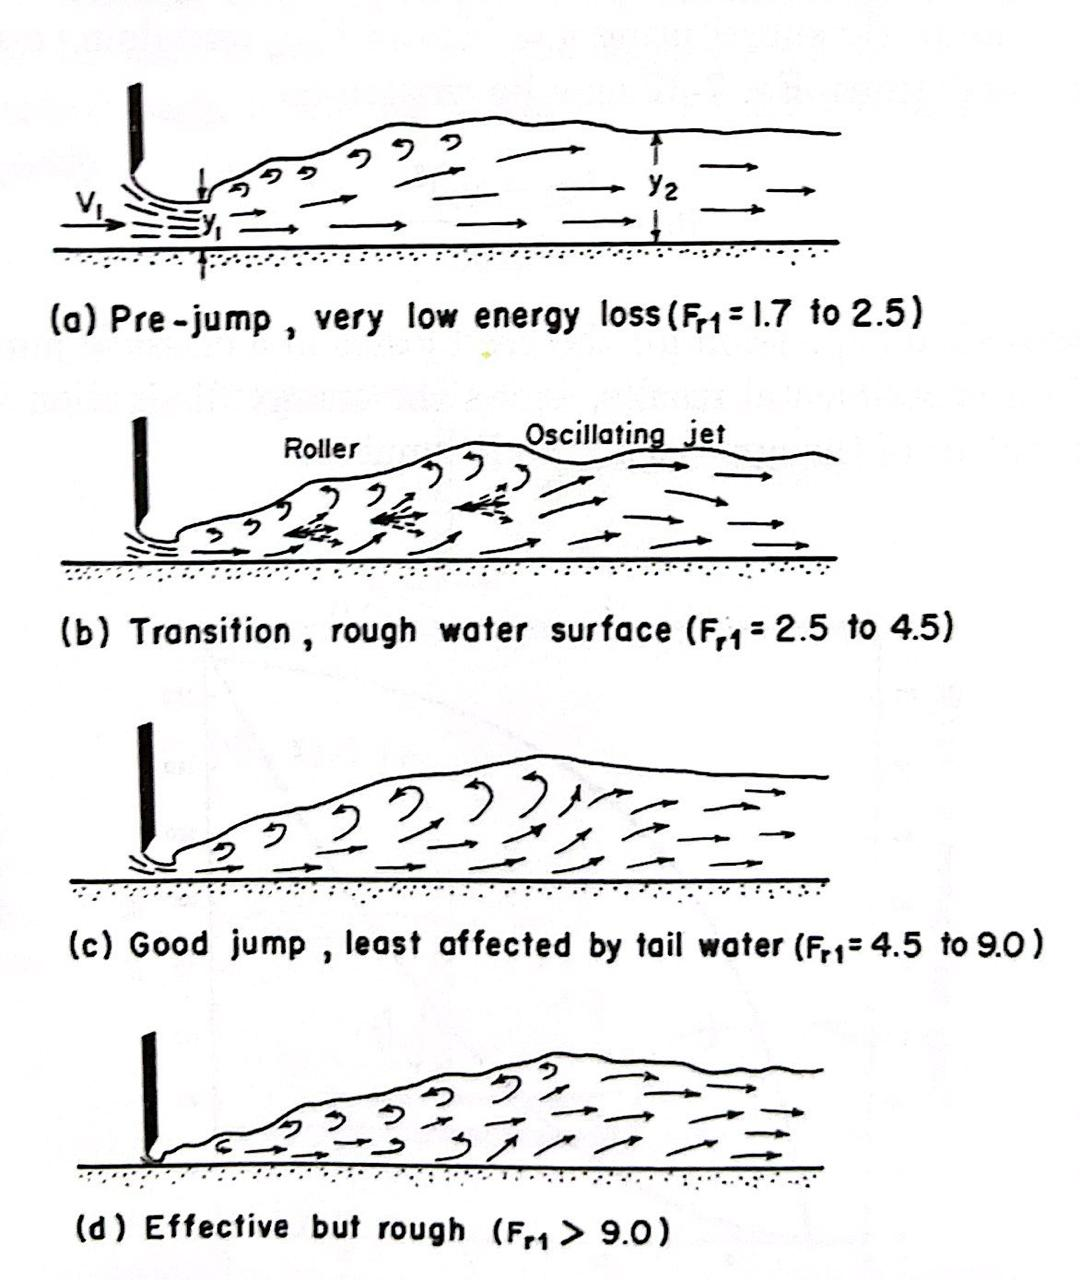
\includegraphics[width=0.8\textwidth]{fig711.jpeg}
\caption{Tipos de resalto hidráulico (tomado de \cite{Chau}).}
\label{fig15}
\end{figure}

\begin{enumerate}
\item \emph{Resalto d\'ebil ($1 < F_{r_1} < 2.5$)}: Poca perdida de energ\'ia y $y_1$ y $y_2$ son aproximadamente iguales.
\item \emph{Resalto oscilante ($2.5 < F_{r_1} < 4.5$)}: Formaci\'on de ondas en la superficie que persisten aguas abajo del resalto. Se debe evitar en el diseño de disipadores.
\item \emph{Resalto permanente ($4.5 < F_{r_1} < 9$)}: El resalto  permanece en su lugar y es menos sensible a cambios en las condicione en la secci\'on 2. Alta disipaci\'on de energ\'ia.
\item \emph{Resalto fuerte ($ F_{r_1} > 9$)}: La diferencia de $y_1$ y $y_2$ es alta as\'i como la disipaci\'on de energ\'ia.
\end{enumerate}

\item \textbf{P\'erdida de energ\'ia}: Las p\'erdidas en un resalto hidr\'aulico para una canal horizontal y rectangular se pueden expresar como:
$$
\Delta E = E_1 - E_2 = y_1 - y_2 + \frac{V_1^2}{2g} - \frac{V_2^2}{2g}
$$

reagrupando y reemplazando de acuerdo a $V=\frac{Q}{A}$, se tiene:
$$
\Delta E = y_1 - y_2 + \frac{Q^2}{2g}\left(\frac{A_2^2 - A_1^2}{A_1^2 A_2^2} \right)
$$

reagrupando nuevamente:
$$
\Delta E = y_1 - y_2 + \frac{Q^2}{2g}\left(\frac{(A_2 - A_1)(A_2 + A_1)}{(A_1 A_2)(A_1 A_2)} \right)
$$

de la ecuaci\'on de fuerza espec\'ifica para el resalto hidr\'aulico ($F_{s_1} = F_{s_2}$), se tiene que $\frac{Q^2}{g} \left(\frac{A_2 - A_1}{A_1 A_2} \right) = \bar{z_2}A_2 - \bar{z_1}A_1 $. Reemplazando en la ecuaci\'on anterior se tiene:

$$
\Delta E = y_1 - y_2 + \frac{(\bar{z_2}A_2 - \bar{z_1}A_1) (A_2 + A_1)}{2 A_1 A_2}
$$

reemplazando $\bar{z}=y/2$ y $A=by$, y simplificando, se tiene:

$$
\Delta E = y_1 - y_2 + \frac{(y_2^2 - y_1^2) (y_2 + y_1)}{4 y_1 y_2}
$$

haciendo operaciones algebr\'aicas y agrupando:

\begin{equation}
\color{red}\boxed{\color{black} \Delta E = \frac{(y_2 - y_1)^3}{4y_1 y_2}}
\label{ene23}
\end{equation}
\end{itemize}

% Eje 2-3 Chau
\begin{eje}{}{eje3}
    Un resalto hidraulico es formado en un canal rectangular horizontal de 5 m de ancho aguas abajo de una compuerta. Si la profundidad de flujo justo aguas abajo de la compuerta es 2 m y el caudal transportado es 150 m$^3$ s$^{-1}$, determinar: a) la profundidad aguas abajo del resalto, b) la longitud del resalto y c) la p\'erdida de energ\'ia en el resalto.
\end{eje}


% REFERENCES
\bibliographystyle{plain} % We choose the "plain" reference style
\bibliography{refs} % Entries are in the refs.bib file

\end{document}
